\documentclass[10pt,twocolumn,letterpaper]{article}
\usepackage{wacv}
\usepackage{times}
\usepackage{epsfig}
\usepackage{graphicx}
\usepackage{amsmath}
\usepackage{amssymb}
\usepackage{subfig}
\usepackage{graphicx}
\usepackage{amsmath}
\usepackage{amssymb}
\usepackage{mathtools} % mathtools builds on and exten0))ds amsmath package
\usepackage{algpseudocode}	% http://ctan.org/pkg/algorithmicx% Include other packages here, before hyperref.
\usepackage{comment, url}
\usepackage[ruled, vlined, linesnumbered]{algorithm2e}
\newcommand{\forceindent}{\leavevmode{\parindent=1em\indent}}
\usepackage[hidelinks]{hyperref}

% Include other packages here, before hyperref.

% If you comment hyperref and then uncomment it, you should delete
% egpaper.aux before re-running latex.  (Or just hit 'q' on the first latex
% run, let it finish, and you should be clear).
%\usepackage[pagebackref=true,breaklinks=true,letterpaper=true,colorlinks,bookmarks=false]{hyperref}

%\wacvfinalcopy % *** Uncomment this line for the final submission

\def\wacvPaperID{****} % *** Enter the wacv Paper ID here
\def\httilde{\mbox{\tt\raisebox{-.5ex}{\symbol{126}}}}

% Pages are numbered in submission mode, and unnumbered in camera-ready
\ifwacvfinal\pagestyle{empty}\fi
\setcounter{page}{1}
\begin{document}

%%%%%%%%% TITLE
\title{{\it E}nKCF: Ensemble of Kernelized Correlation Filters for
  High-Speed Object Tracking}

% Authors at the same institution
%\author{First Author \hspace{2cm} Second Author \\
%Institution1\\
%{\tt\small firstauthor@i1.org}
%}
% Authors at different institutions
\author{First Author \\
Institution1\\
{\tt\small firstauthor@i1.org}
\and
Second Author \\
Institution2\\
{\tt\small secondauthor@i2.org}
}

\maketitle
\ifwacvfinal\thispagestyle{empty}\fi

%%%%%%%%% ABSTRACT
\begin{abstract}
Computer vision technologies are very attractive for practical
applications running on embedded systems. This is primarily because
most of embedded systems come with an image acquisition pipeline, and
a tremendous amount of progresses on computer vision research has been
made for the past few decades. However, to successfully deploy a
computer vision algorithm on any existing embedded systems, a vision
algorithm needs to satisfy, at least, two criteria with the assumption
of reasonably good performance: minimal, manual intervention after
deployment and small footprint of consuming computational
resources. Kept these criteria in mind, to develop a single, target
tracking system, we propose an ensemble of the kernelized correlation
filters (KCF), we call {\it E}nKCF. This committee of KCFs is
specifically designed to address the scale-change and dynamic maneuver
of the target over frames. In particular, to guarantee a high-speed,
run-time performance, we deploy each of KCFs in turn, instead of
applying multiple KCFs on each frame. To minimize any potential drifts
between individual KCFs' transition, we developed a Bayes
filter. Experimental results showed that the performance of ours are,
on average, 70.10\% for precision at 20 pixels, 53.00\% for success
rate for OTB100 data, and 54.50\% and 40.2\% for UAV123 data. These
results showed that our method is better than existing ones over 5\%
on precision on 20 pixels and 10-20\% on AUC on average. Moreover our
implementation ran at 340 fps for OTB100 and at 416 fps for UAV123
data that is faster than DCF (292 fps) for OTB100 and KCF (292 fps),
DCF (457 fps) for UAV123. To increase flexibility of the proposed {\it
  E}nKCF running on various single-board computers, particularly, ones
with GPUs, we explored different levels of deep features.
\end{abstract}

%%%%%%%%% BODY TEXT
\section{Introduction}
A recent advancement of air/ground/water unmanned vehicle technologies
has increased interests on deploying intelligent algorithms to
existing embedded and mobile platforms. Among those technologies,
computer vision algorithms are getting more attentions primarily
because payloads of those mobile platforms are limited to carry any
other sensors than a monocular camera. Instead of just manually being
flew for video recording, an unmanned air vehicle (UAV) equipped with
an object or feature following functionality would make it more useful
in the application of monitoring/surveillance/surveying on private
properties/wild-life/crop, video recording on sports/movies/events,
many others.

\begin{figure*}[!h]
\centering
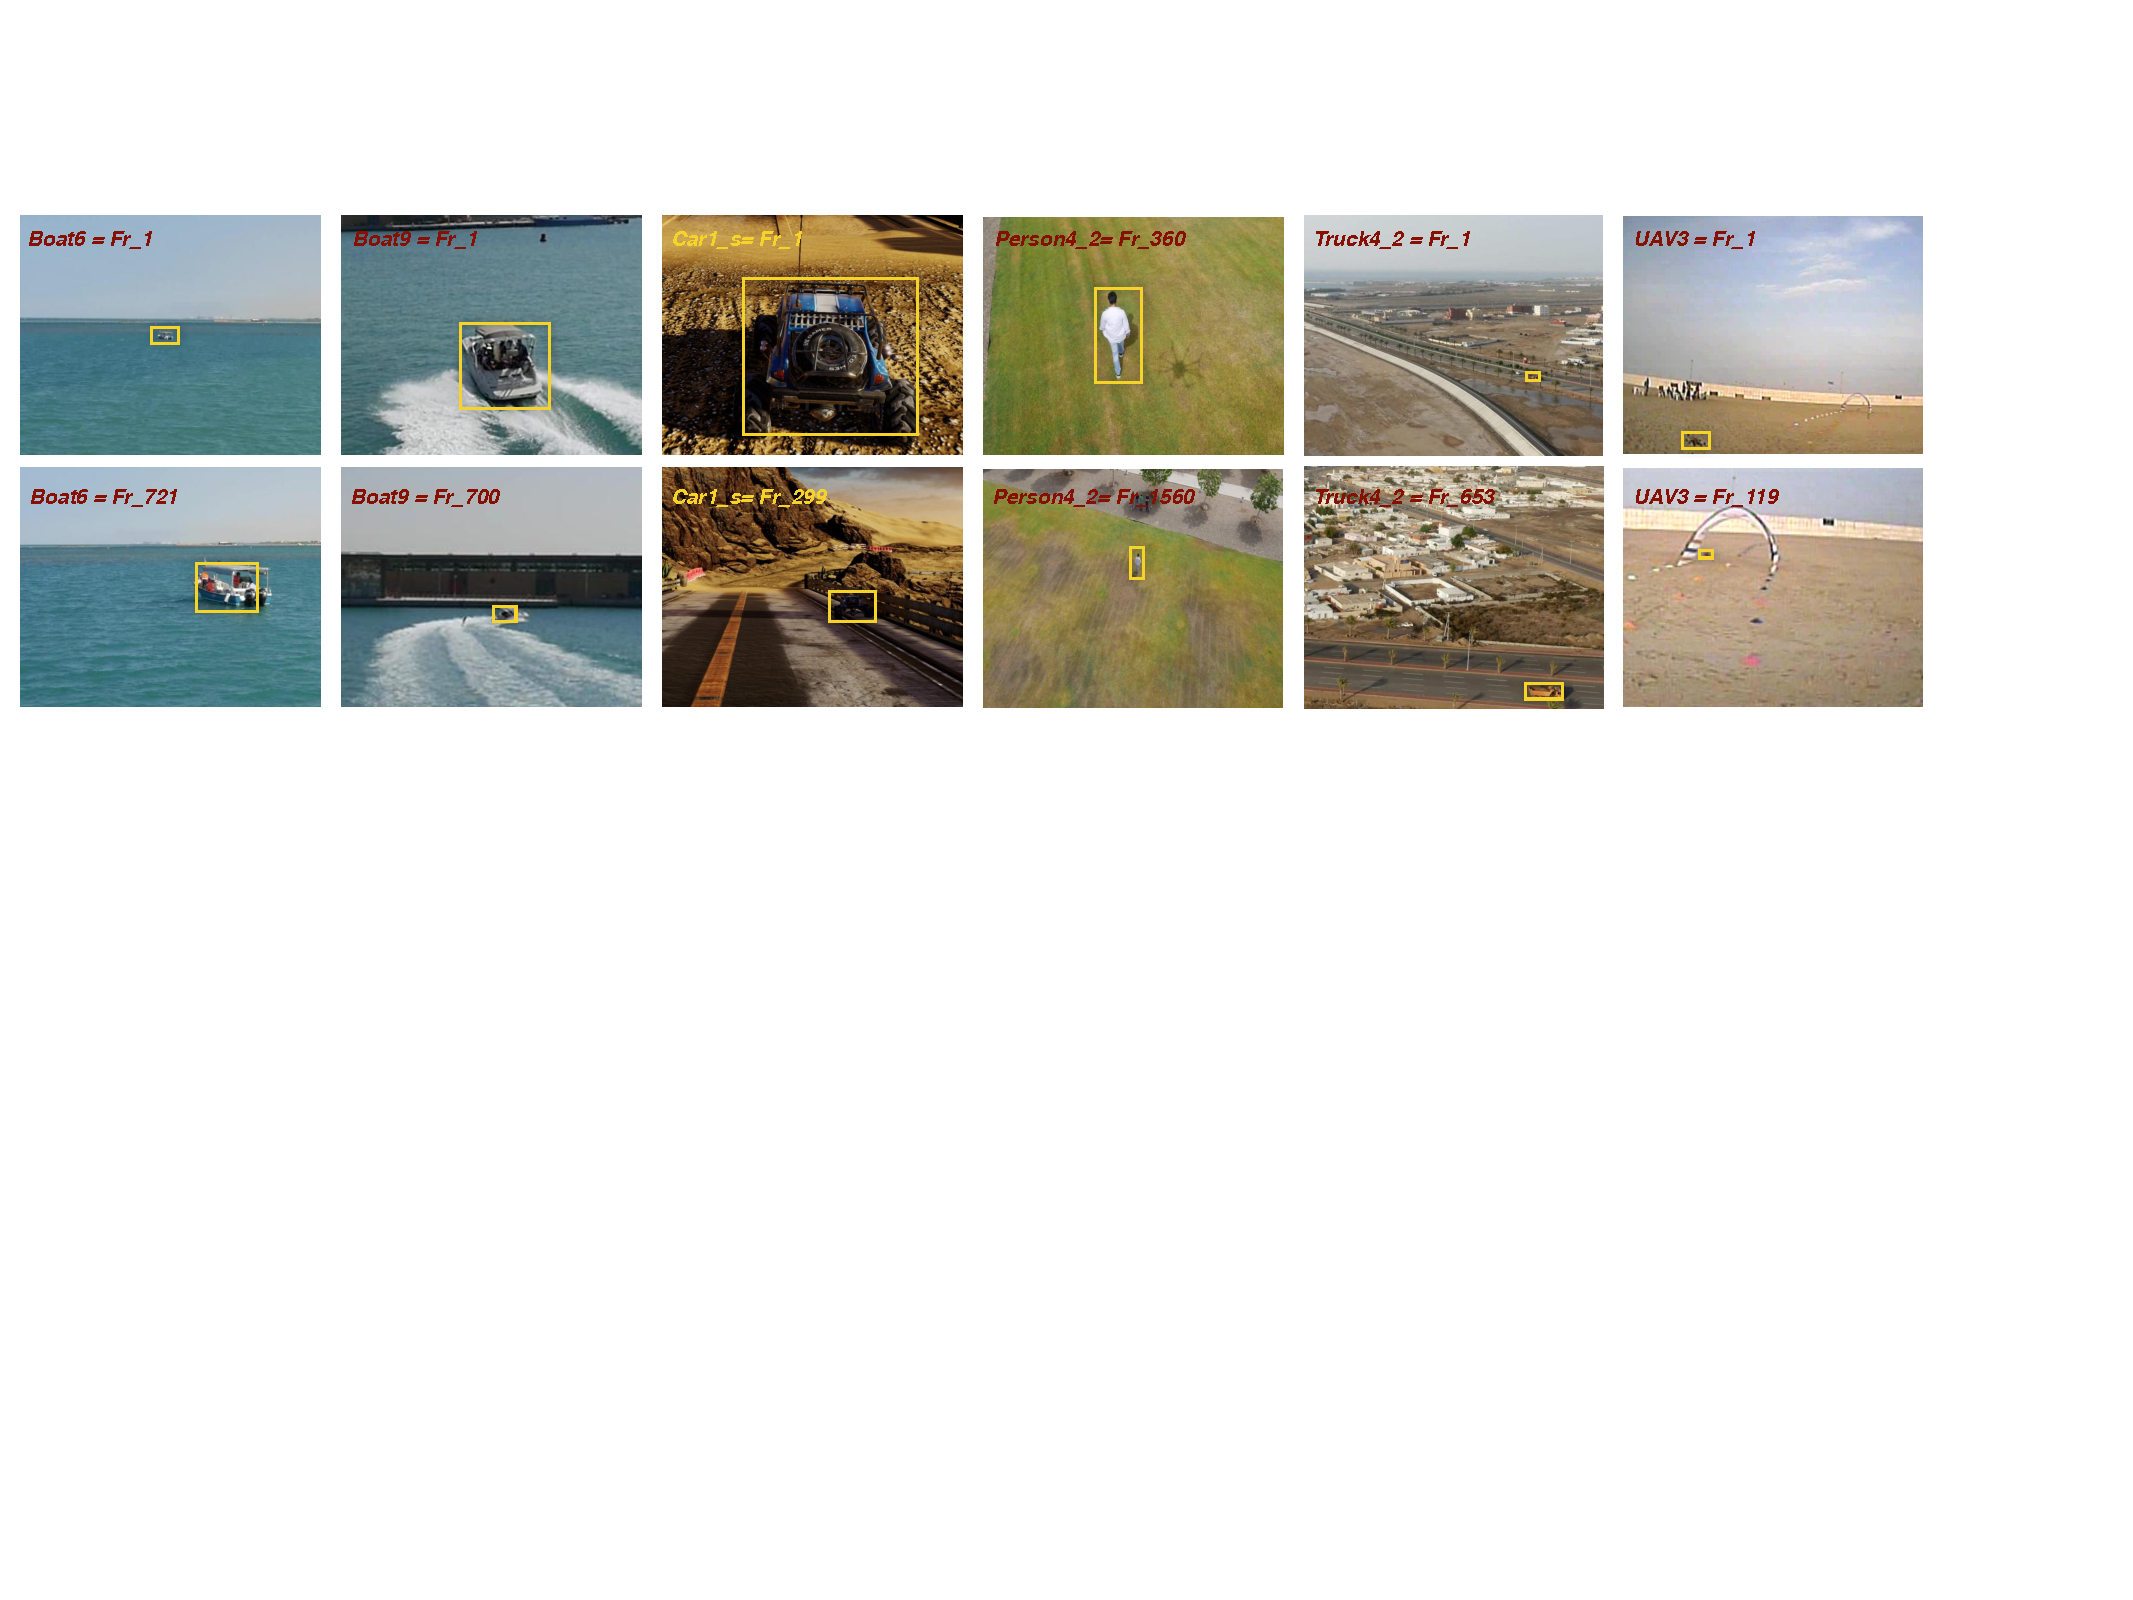
\includegraphics[width=\textwidth]{./figures/ResultsIntroduction.pdf}
\caption{Examples of tracking results (yellow rectangles) by the
  proposed method on the ``UAV123'' dataset. This ``UAV123'' dataset
  is challenging for object tracking as a target's scale is changed
  drastically in a few frames.}
\label{ResultsIntroduction}
\end{figure*}

In this paper, we propose a single-target tracking algorithm that does
not require offline training and can run on any embedded or mobile
platforms. Specifically, we would like to make our algorithm 1) learn
the appearance model of a target on the fly and 2) run as fast on a
typical desktop as up to $300$-$450$ fps, aiming at running, at least,
faster than 30 fps when it is deployed on a low-end, embedded
system.\footnote{In general, it would not be easy to compare run-time
  performance of a computer vision algorithm at an Intel or AMD
  processor running on a desktop or a laptop and at that (e.g., ARM)
  of a single-board, embedded system. This is primarily due to the
  difference in their architectures and available computing
  resources. To derive these numbers (300 and 30 fps), we assume that
  there is roughly, at least, an 1/10th scale down of computational
  resources from a typical PC to an embedded system. We found such a
  scale-down in computation based on exemplar processors, e.g.,
  Intel's i7 quad-core vs ARMv8 dual-core.}

\begin{figure*}[!h]
\centering
\begin{tabular}{cc}
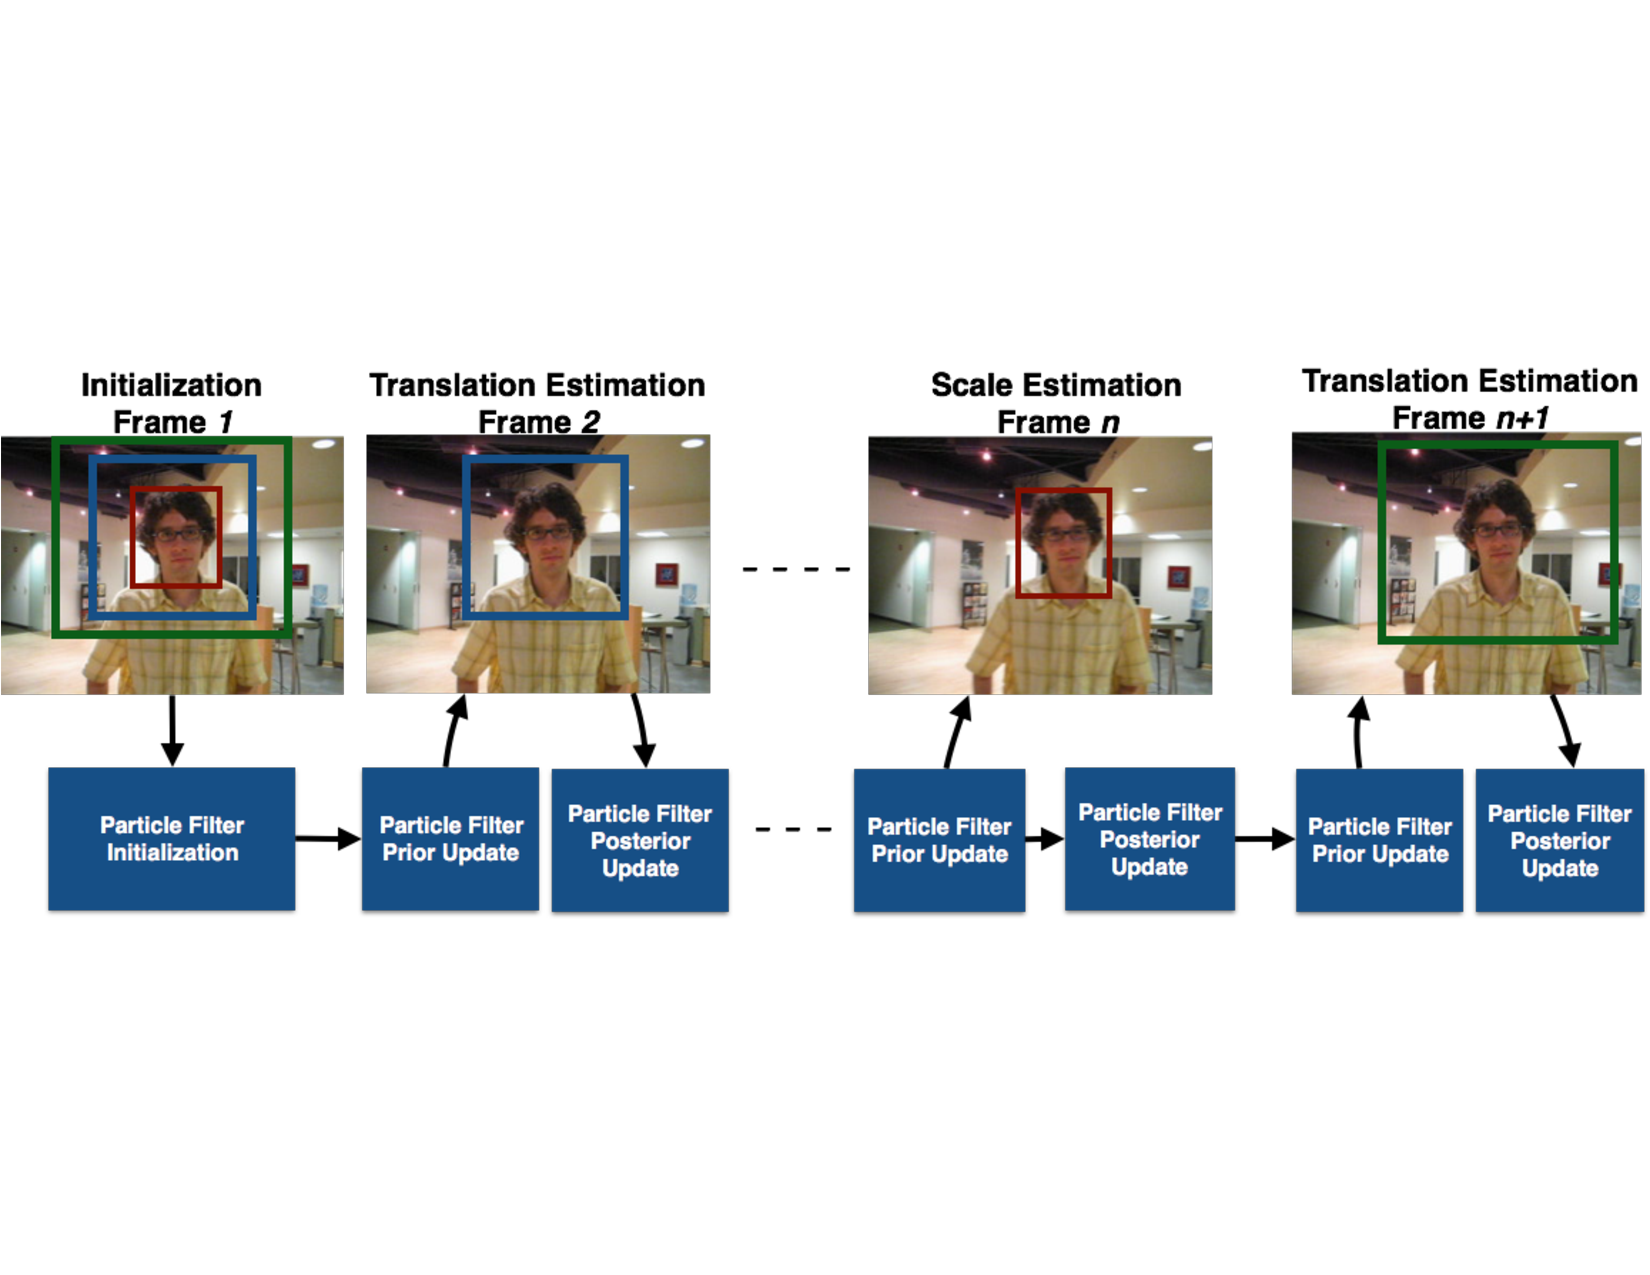
\includegraphics[width=14.00cm]{./figures/Workflow_MKCF+PF.pdf}\\
\end{tabular}
\caption{The work-flow of the proposed single-target tracking
  algorithm, {\it E}nKCF. We show the first seven frames of tracking
  where the first frame is the initialization frame. Afterward, the
  order of deploying three KCFs is repeating.}
\label{Workflows}
\end{figure*}

One of the dominant frameworks for online object tracking is the
correlation filter that essentially solves a single-target tracking
problem as a regression problem in the frequency domain. This
framework assumes that a target location is given at the beginning
like any other online tracking algorithms
\cite{smeulders2014survey}. Given this positive example for the
regression problem, a set of negative examples is collected around the
initial, target bounding box and represented as a form of the
circulant matrix \cite{henriques2015high}. One can optimally solve
this regression problem using a ridge regression in a closed
form. However, this solution involves in expensive matrix operations
$\mathcal{O}(n^{3})$. The correlation filter offers a less complex
solution, $\mathcal{O}(n\log n)$ over element-wise multiplication in a
frequency domain \cite{bolme2010visual,henriques2015high}. Thank to
this reformulation, an object tracking pipeline based on the
correlation filter can run very efficiently and be even easily
implemented. In fact, an extension of a linear correlation filter, the
kernelized correlation filter with multi-channel features
\cite{henriques2015high} showed impressive object tracking results and
outperformed other state-of-the-art, online tracking algorithms in
terms of run-time and tracking accuracy. However, a vanilla form of
such an online tracker is prone to drift, and fails to track a target
over a long period of time \cite{henriques2015high}. This is primarily
due to the dilemma of stability-plasticity in updating appearance
model, where the appearance model will be overfitted to only the
images used to train, unless a compromise on the frequency of updating
the model is carefully implemented \cite{santner2010prost}. For
example, one may handle a target's scale variation by just
concatenating multiple correlation filters including KCF and running
them on each frame. Alternatively one could think of scanning the
region of interest (ROI) with a list of templates in predefined scale
ratios to find the target in appropriate scale
\cite{henriques2015high,tang2015multi,ma2015long,bibi2015multi,li2014scale}. However,
these approaches will drastically reduce run-time performance because
they are proposed to run multiple KCF on each frame.

Another way of handling the scale change for the correlation filter
based approach is to estimate a correct scale at a location where a
target highly likely appears \cite{zhang2014fast} -- estimate a
target's translation first and estimate a correct scale afterward. In
particular, Zhang and his colleagues use the MOSSE tracker \cite{bolme2010visual} to 
estimate the target's translation. And then they attempted to update the scale of
the target by further analyzing image, sub-regions with high
confidence. This is based on an assumption that the scale of a target
would not change much over two consecutive frames. Similarly, Ma and
his colleagues used two KCFs to learn the translation and scale of a
target separately \cite{ma2015long}. In particular, a KCF is used to
learn the translation of the target and its background. Given this,
another KCF is used to learn the target area to estimate a new scale
of the target. However, because of running more than a KCF on each
frame, this method degrades its run-time performance (i.e., $\leq 50
fps$). Our method is motivated by this idea -- the idea of deploying
multiple KCFs to address the issues of single target tracking: scale
and translation, but in a more efficient way. To maximize run-time
performance and accuracy, instead of running them all together on
every frame, we deploy three KCFs in turn:
\textit{target}+\textit{small background} translation filter
($R_{t}^{S}$), \textit{target-only} scale filter ($R_{s}$) and
\textit{target}+\textit{large background} translation filter
($R_{t}^{L}$). By doing so, our method aims at addressing a scale
change and estimate target's motion efficiently while maintaining or
increasing run-time performance. Figure \ref{Workflows} illustrates
the work-flow of the {\it E}nKCF.

The contribution of this paper is a novel, single-target tracking
algorithm running in a very high-speed ($\geq300$ fps), that deploys an
ensemble of KCFs, in turn, to more effectively address the scale
variance and the dynamic maneuver of a target while preserving
run-time performance as high as possible. We also developed a Bayes
filter to minimize any potential drifts while transiting one KCF to
another. In addition, we explore deep features with varying levels of
abstraction in the proposed {\it E}nKCF to improve tracking
performance and increase its flexibility being deployed on high-end,
single-board computer with GPUs.

%---------------------------------------------------------------------- 
\section{{\it E}nKCF: Ensemble of Kernelized Correlation Filters}
%---------------------------------------------------------------------- 

We propose a novel way of utilizing a multiple of the KCFs
\cite{henriques2015high} to effectively handle scale variations and
dynamic maneuvers of a target. To maintain or improve the run-time
performance of the original KCF (e.g., $\ge$ 300), we deploy three
KCFs in turn, instead of applying them on the same image frame
together. Each of these KCFs is designed to address specific
challenges: scale and translation. By alternating their deployments,
our algorithm will improve the performance of the original KCF while
preserving the efficient nature and small-footprint of the KCF
computation.

\begin{algorithm*}[h]
\small
\DontPrintSemicolon
\KwIn{ Initial bounding box $(x_{0},y_{0},s_{0})$, frame counter $fc$, complete cycle of scale filter $n = 5$,}
\KwOut{	\uIf{$fc\:\%\:n=0$ (\textbf{Condition 1})}
			{
				Estimated Target State $(x_{t},y_{t},s_{t})$,
				Scale filter (\textit{target-only}) model $R_{s}$
			}
			 \ElseIf{$fc\:\%\:n>0\:\:and\:\:fc\:\%\:n\leq n/2$ (\textbf{Condition 2})}
			 {
				Estimated Target State $(x_{t},y_{t},s_{t} = s_{t-1})$,
			  	Large Area Translation Filter model $R_{t}^{L}$
			}			 
			 \Else (\textit{\textbf{Condition 3}})
			{			 
				 Estimated Target State $(x_{t},y_{t},s_{t} = s_{t-1})$,
				Small Area Translation Filter model $R_{t}^{S}$			
			}	
		}
\SetKwBlock{Begin}{function}{end function}
\Begin($\text{track($x_{t-1},y_{t-1},s_{t-1}$) }$)
{
 	// \textit{Translation Estimation - Particle Filter} \\
	Transit Particle Filter to the frame $t$ and compute the mean of prior pdf $\mathbf{(x_{t},y_{t},s_{t-1})}$ \\
     // \textit{Translation Estimation - Correlation Filter} \\
	Crop the ROI for the $R_{t}^{L}$ (Condition 2), or $R_{t}^{S}$ (Condition 3) given $(x_{t},y_{t})$ and estimate new position as $\mathbf{(x_{t},y_{t})}$ = $\mathbf{\textit{max}(y_{R_{t}})}$\\
	// \textit{Scale Estimation - Correlation Filter}\\
	Scale pool for $R_{s}$ : $S = \lbrace1.05,1.0,1/1.05\rbrace$,\\
	Crop the ROI for the $R_{s}^{i}$ (Condition 1) and estimate scale factor, $\mathbf{\alpha}$ = $\mathbf{\underset{i\in S}{\textit{argmax}}(PSR(y_{R_{s}^{i}}))}$, and new scale $\mathbf{s_{t} = \alpha * s_{t-1}}$,\\ 
	Skip it for $R_{t}^{L}$ and $R_{t}^{S}$ ($\mathbf{s_{t}}$=$\mathbf{s_{t-1}}$)\\
	// \textit{Update Translation - Particle Filter}\\
	Do Importance Re-sampling (if necessary) and compute the 
	mean of posterior pdf $\mathbf{(x_{t},y_{t})}$\\
	// \textit{Model Update}\\
	Update $R_{t}^{S}$,\\
	Update $R_{t}^{L}$\\
	\uIf{$PSR(y_{R_{s}}) \geq T_{R_{s}}$}{
		Update $R_{s}$ (Condition 1)}
  \label{endfor}
  \Return{($x_{t},y_{t},s_{t}$)}
}
\caption{{\it E}nKCF Tracking Algorithm}\label{alg:MKCF}
\end{algorithm*}

The proposed algorithm, {\it E}nKCF, learns three KCFs in turn: The
first filter, $R_{t}^{S}$, focuses on learning the target area and its
background, \textit{target}+\textit{small background} for addressing a
marginal translation by a target, the second filter, $R_{s}$, focuses
entirely on learning the target's scale, \textit{target-only}, and the
last filter, $R_{t}^{L}$, focuses on the target area and its
background bigger than that of the first filter, $R_{t}^{S}$,
\textit{target}+\textit{large background}. We set up {\it E}nKCF in
this way because, we believe, a correlation filter for learning a
target's translation should include the background of the target to
better discriminate it from its surrounding, and another correlation
filter should focus on the target itself to estimate the right scale
of the target. By setting a transition filter with larger padding
size, $R_{t}^{L}$, we can recover from potential drifts after the
frames we only run the scale filter. Additionally, we design a
translation filter with smaller padding size, $R_{t}^{S}$, to better
localize the position of the target after the frames we only run
$R_{t}^{L}$.

Our approach is similar to that of \cite{ma2015long} in that more than
one KCF is used to address the challenges of single target
tracking. But ours is different from their approach because we do not
use those multiple KCFs together at every frame, but alternatively at
every $k$ frame. It intuitively makes sense to alternatively use
multiple KCFs with different purposes because the appearance of a
target does not change drastically over consecutive image frames. For
most case, even it looks the appearance changes, learning a
correlation filter over consecutive frames would not be substantially different
from the one learned using the image few or $k$ frames later. Figure
\ref{fig:Filters_Comparison} shows examples supporting this
observation.

\begin{comment}
Since Henriques and his colleagues' presented impressive tracking
results of KCF \cite{henriques2015high} on VOT15
challenge \footnote{\url{http://www.votchallenge.net/vot2015/}}, many
variation of KCF were investigated. For example, \cite{ma2015long} and
\cite{danelljan2014accurate} used a scale filter to learn the target
area only whereas \cite{li2014scale, bibi2015multi, tang2015multi}
used a correlation filter learned on the target area and its
surrounding background in different size to learn the optimal scale of
the target. Our approach is similar to that of \cite{ma2015long} in
that more than one KCF is used to address the challenges of single
target tracking. But ours is different from their approach because we
do not use those multiple KCFs together at every frame, but
alternatively at every $k$ frame. It intuitively makes sense to
alternatively use multiple KCFs with different purposes because the
appearance of a target does not change drastically over consecutive
image frames. For most case, even it looks the appearance changes,
learning a correlation filter over consecutive frames would not be
much different from the one learned using the image few or $k$ frames
later. Figure \ref{fig:Filters_Comparison} shows examples supporting
this observation.
\end{comment}

\begin{figure*}[!h]
\centering
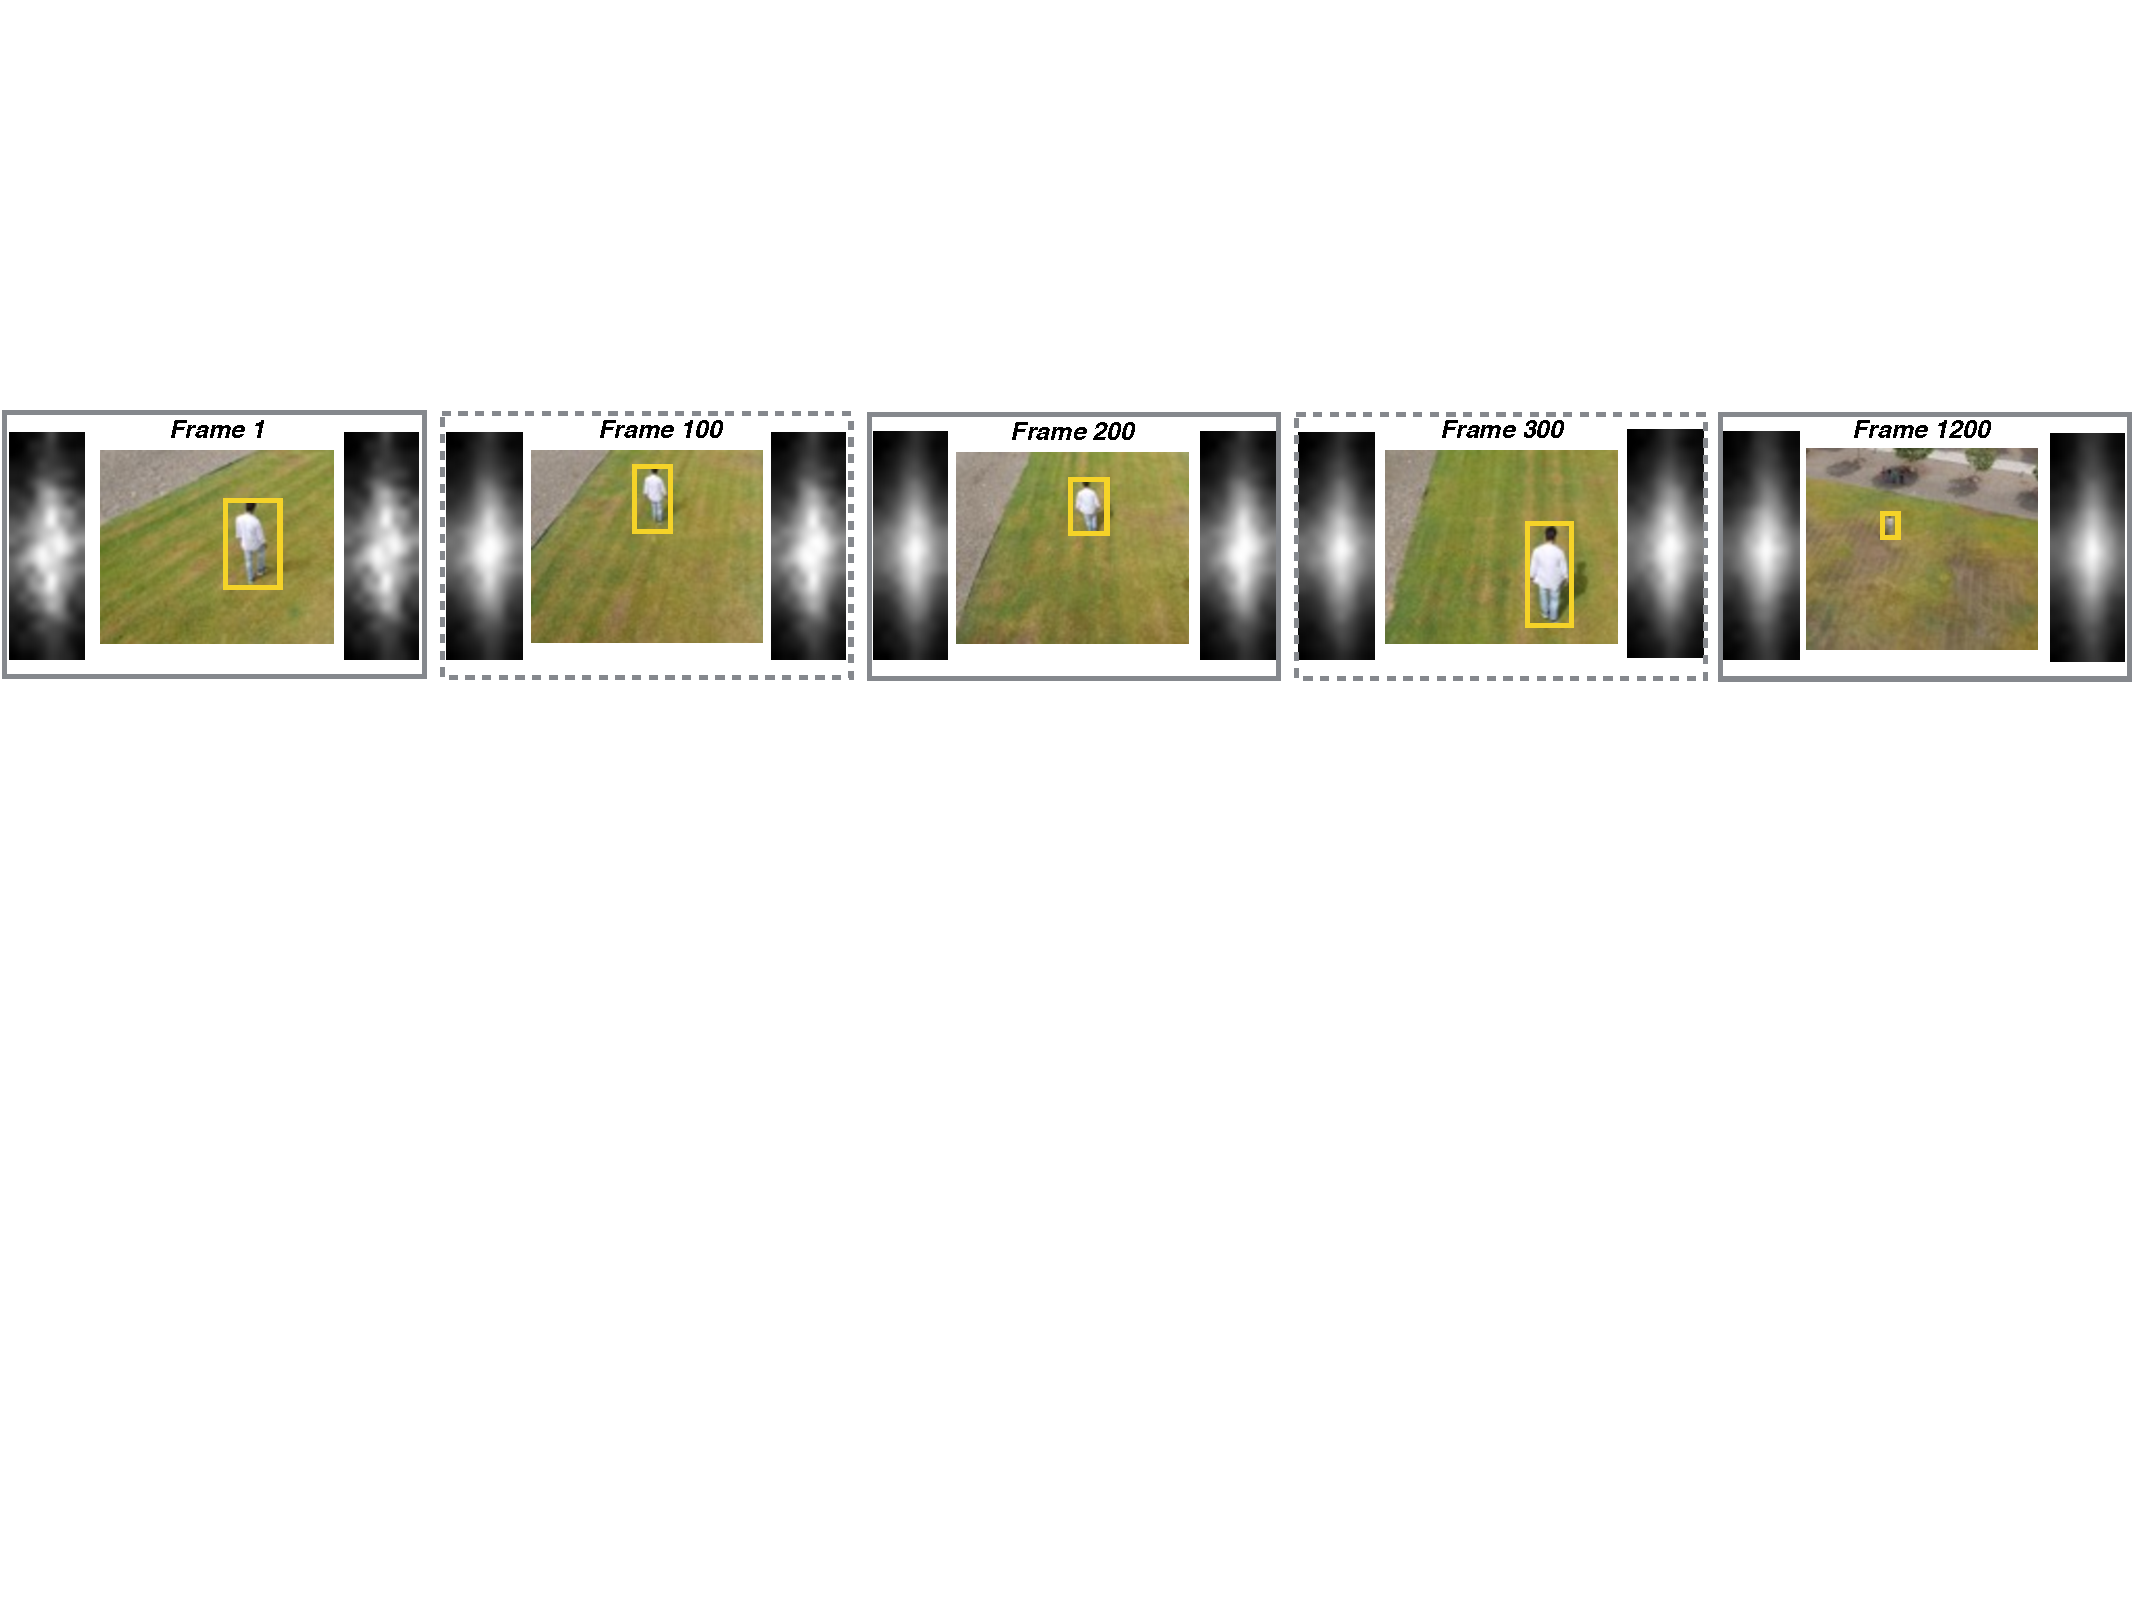
\includegraphics[width=1\textwidth]{./figures/LearnedFiltersComparison2.pdf}
\caption{This figure shows that there is a marginal difference among
  the scale filters learned either at every frame or at every 5
  frames. The sub-figures at the the left show the scale filters
  trained at every frame and those at the right show the scale filters
  trained at every 5 frames.}
\label{fig:Filters_Comparison}
\end{figure*}

The algorithm \ref{alg:MKCF} shows the pseudo-code of {\it E}nKCF.
The order of running these three KCFs is important because each of
these filters aims at addressing different challenges. The
\textit{target+large background} translation filter, $R_{t}^{L}$, is
applied to the $i$th and $i$+$1$th image frames, another translation
filter, $R_{t}^{S}$ is applied to the $i$+$2$th and $i$+$3$th image
frames, and then the scale filter, $R_{s}$ is applied to the
$i$+$4$the image. This order repeats until the end of the image
frames. The translation filter, $R_{t}^{L}$, is intended to run right
after the scale filter, $R_s$, runs which is applied at every other
$i$+$4$ frames. We run these filters in this way because we want to
minimize any drifts that are likely to happen running only $R_{s}$. In
addition, the filter, $R_{t}^{S}$, is applied to every other two
frames before $R_{s}$ and right after two consecutive frames running
$R_{t}^{L}$. By repeating this order of learning KCFs, we can
integrate more discriminative shape features that cannot be learned
just by $R_{t}^{L}$. The filter, $R_{t}^{L}$, uses shape and color
information together to recover from any potential drifts -- drifts
could happen only looking the target's scale by the filter, $R_{s}$.

In summary, the scale filter, $R_{s}$, is designed to directly handle
the scale change of a target and provides other translation filters
$R_{t}^{L}$ and $R_{t}^{S}$ with more focused ROIs about the target's
translation. On the other hand, a translation filter, $R_{t}^{L}$, is
designed to look at a larger search area to estimate the target's
translation and recover from any potential drifts. Another translation
filter, $R_{t}^{S}$, is designed to addresses the drawback of
$R_{t}^{L}$ that it may learn noisy shape features due to its large
search area. In what follows, we will detail the main idea behind the
KCF.

\textbf{Kernelized Correlation Filter} The Kernelized Correlation
Filter is a well-known single target tracking method and its work
flow has been detailed in other papers
\cite{henriques2012exploiting,henriques2015high}. This section briefly
goes over the parts of the KCF relevant to this study. Its
computational efficiency is derived from the correlation filter
framework representing training examples as a circulant matrix. The
fact that a circulant matrix can be diagonalized by Discrete Fourier
transform is the key to reduce the complexity of any tracking method
based on correlation filter. The off-diagonal elements become zero
whereas the diagonal elements represent the eigenvalues of the
circulant matrix. The eigenvalues are equal to the DFT transformation
of the base sample ($\mathbf{x}$) elements. The Kernelized Correlation Filter,
in particular, applies a kernel to $\mathbf{x}$ to transform to a more
discriminative domain. The circulant matrix is then formed by applying
cyclic shifts on the kernelized $\mathbf{x}$. Such kernelization operation
maintains O($nlog(n)$) complexity unlike other kernel algorithms
leading to O($n^{2}$) or even higher complexities.

The KCF solves essentially the problem of a regression in the form of
the regularization (ridge regression):
\begin{equation}
E(h) = \frac{1}{2}||\mathbf{y}-\sum_{c=1}^{C}\mathbf{h_{c}}*\mathbf{x_{c}}||^{2} + \frac{\lambda}{2}\sum_{c=1}^{C}||\mathbf{h_{c}}||^{2}
\label{eq:Closedform_RidgeReg}
\end{equation}
where $\mathbf{y}$ represents the desired continuous response whereas $\mathbf{h}$ and
$\mathbf{x_{c}}$ represents the learned correlation filter and training
template for the given channel. The parameter $c$ enabled one to
integrate features in multiple channels, such as HoG and color, in
this setup \cite{henriques2015high,galoogahi2013multi}. A closed-form
solution for Equation \ref{eq:Closedform_RidgeReg} exists. To simplify the
closed-form solution, an element-wise multiplication in
frequency domain was proposed for $\hat{w}$:
\begin{equation}
\mathbf{\hat{w}} = \mathbf{\hat{x}^{*}}*\mathbf{\hat{y}}(\mathbf{\hat{x}^{*}}*\mathbf{\hat{x}}+\lambda)^{-1}.
\label{eq:DiagonalizedPrimalSolution}
\end{equation}
A non-linear version of this closed-form solution is proposed to increase robustness
to any geometric and photometric variations
\cite{henriques2015high}. In particular, the diagonalized Fourier
domain dual form solution is expressed as
\begin{equation}
\mathbf{\hat{\alpha}} = \mathbf{\hat{y}}(\mathbf{\hat{k}^{xx}}+\lambda)^{-1}
\label{eq:FourierDualDomainSolution}
\end{equation}
where $\lambda$ represents the regularization weight whereas $\mathbf{\hat{k}^{xx}}$ denotes
 the first row of the kernel matrix $\mathbf{K}$ known as \textit{gram matrix} and it is expressed as
\begin{equation}
\mathbf{k^{xx^{'}}} = exp(-\dfrac{1}{\alpha^{2}}(||\mathbf{x}||^{2}+||\mathbf{x}^{'}||^{2}-2F^{-1}(\sum^{C}_{c}\mathbf{\hat{x}_{c}}^{*}\odot \mathbf{\hat{x}_{c}}^{'})))
\label{eq:GaussianCorrelationSingleChannel}
\end{equation}
An early version based on this formulation used grayscale feature
($C=1$) to learn the solution vector $\mathbf{w}$ and multi-channel features
such as HoG and Color showed improved accuracy
\cite{henriques2015high,galoogahi2013multi,tang2015multi,ma2015long,bibi2015multi}. 
Specifically, one can execute an object detection task using this kernelized correlation
filter with multi-channel features as
\begin{equation}
\mathbf{r(z)} = F^{-1}(\mathbf{\hat{k}^{xz}} \odot \mathbf{\hat{\alpha}})
\end{equation}
where $\mathbf{r}$ denotes the correlation response at all cyclic shifts of the
first row of the kernel matrix.

In the following sections, we will detail two different types of
features used in {\it E}nKCF : (1) hand-crafted features (fHoG +
color-naming) and (2) deep convolutional features.

\textbf{{\it E}nKCF with Hand-Crafted Features} We, first, use two
conventional hand-crafted features, fHoG (shape)
\cite{felzenszwalb2010object} and color-naming (color)
\cite{li2014scale}. Figure \ref{fig:Filters} shows examples of these
features. This setup of the {\it E}nKCF is designed to perform
tracking on any embedded systems at $30$ fps, ones without GPUs.
\begin{figure}[!h]
\centering
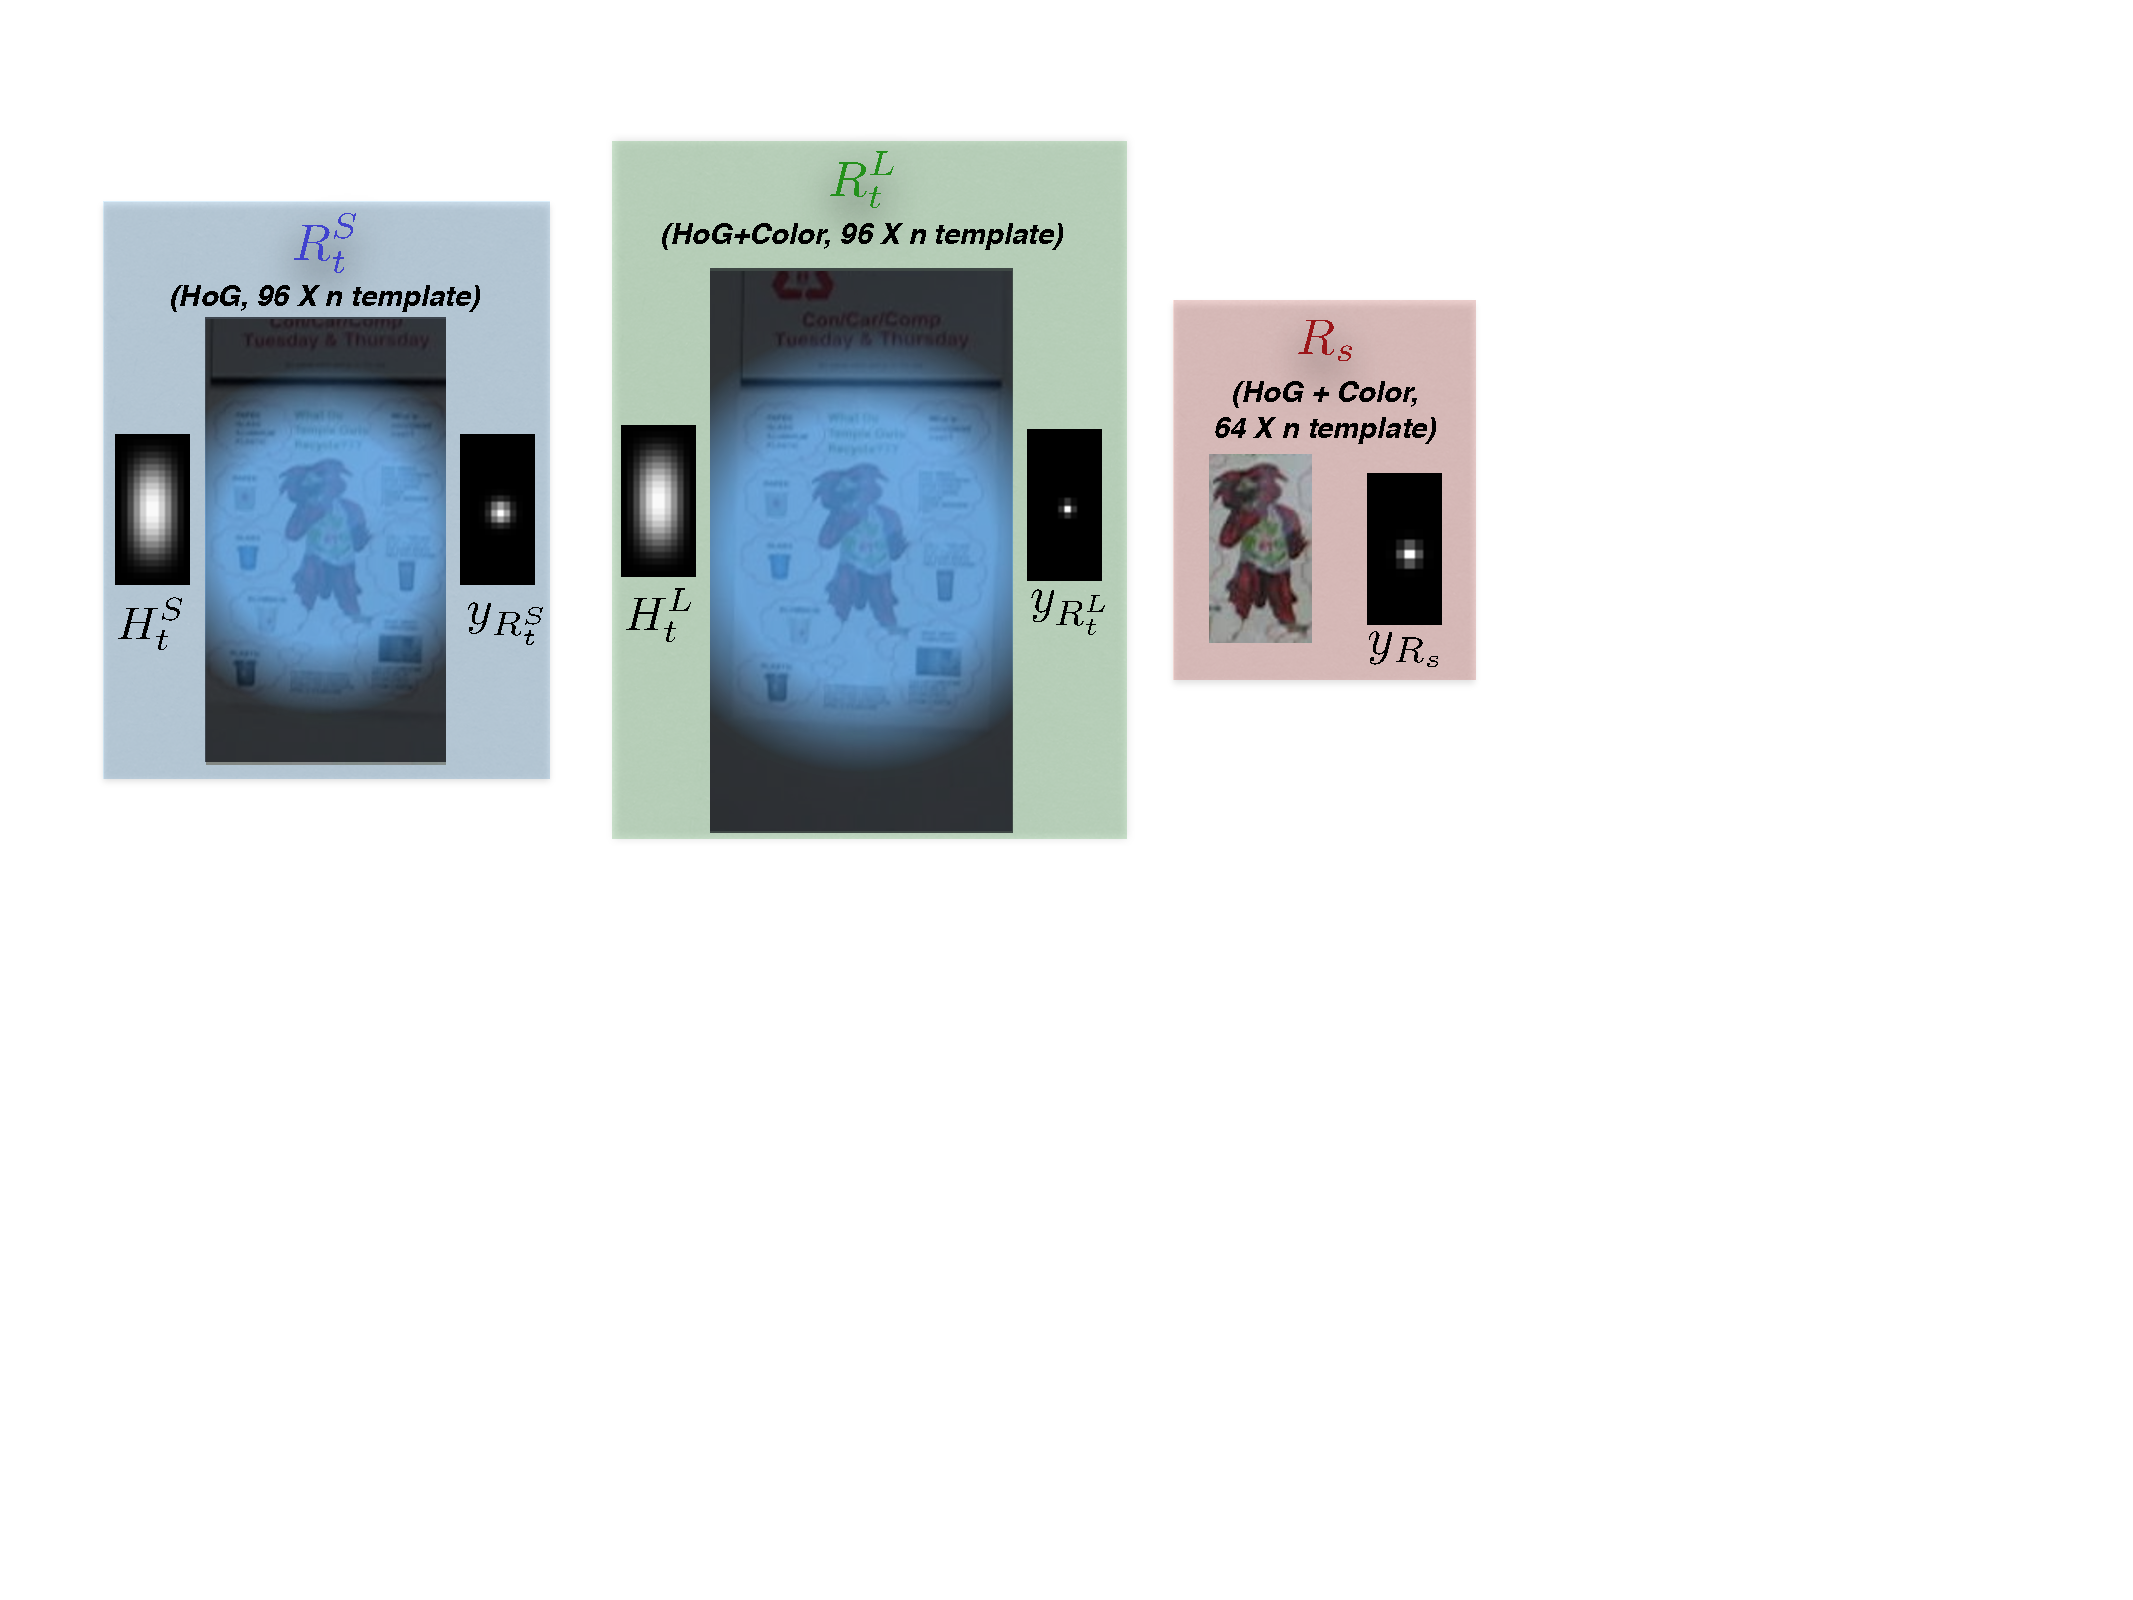
\includegraphics[width=0.47\textwidth]{./figures/Filters_Details.pdf}
   \\[-3ex]
\subfloat[Small Area Translation Filter]{\hspace{.30\linewidth}}\label{fig:Rt_S}
\quad\subfloat[Large Area Translation Filter]{\hspace{.37\linewidth}}\label{fig:Rt_L}
\quad\quad\subfloat[Scale Filter]{\hspace{.12\linewidth}}\label{fig:Rs}
\caption{Examples of three filters with hand-crafted features.}
\label{fig:Filters}
\end{figure}

We use both fHoG \cite{felzenszwalb2010object} and color-naming
\cite{van2009learning} for the large area, translation filter,
$R_{t}^{L}$. This is because the fHoG applied to relatively larger
area tends to be noisy and less discriminative and adding color
information makes the feature vector for the translation filter,
$R_{t}^{L}$, more robust to noise and more discriminative. Figure
\ref{fig:Filters}(b) shows an example of this translation filter. But,
this is not the case for the small area, translation filter,
$R_{t}^{S}$, because it does not contain much of
the background area around the target. For this reason, the $R_{t}^{S}$ only
employs the fHoG features. Figure \ref{fig:Filters}(a)
shows an example of this translation filter. Lastly, we use both fHoG
and color-naming features again for the scale filter,
$R_{s}$. By assigning fHoG and color-naming features, we ensure
that the likelihood of inaccurate scale estimation is reduced in comparison to the scale filter
with only fHoG features. This is more important in our case as the scale filter is operated in every 5 frames
in the proposed tracker. Also, the scale filter, explained earlier in the
algorithm \ref{alg:MKCF}, estimates the scale of a target by
correlating it with three candidate ROIs. This search may increase the
run-time complexity of the scale filter from $\mathcal{O}(n\log n)$ to
$\mathcal{O}(3(n\log n))$. To ensure actual filtering operations
practical, we use a smaller template size (i.e., 64$\times n$) for the
scale filter, $R_{s}$. The smaller template size does not degrade the
tracking performance because of 1) zero padding around the
target (smaller ROI) and 2) use of color-naming features.
\begin{comment}
The ROI considered by $R_{s}$ is resized to a smaller template
resolution ($64\times n$) as shown in Figure~\ref{fig:Filters}(c).
This leads to less discriminative shape features. To reduce the noise
in $R_{s}$, we concatenate color features.  The $R_{s}$ estimates the
scale by correlating the filter with three candidate ROIs as detailed
in algorithm~\ref{alg:MKCF}.  This increases the complexity from
$\mathcal{O}(n\log n)$ to $\mathcal{O}(3(n\log n))$ for $R_{s}$.  To
reduce the number of operations, we assign a smaller template size to
$R_{s}$.  This does not degrade the tracking performance due to two
reasons: (1) zero padding around the target and (2) integration of
color features. This way, we keep the run-time complexity of the
$R_{S}$ similar to $R_{t}^{L}$ and $R_{t}^{S}$ that only run
correlation filter on a single ROI. By reducing the template size of
$R_{s}$, fluctuating run-time performances among $R_{s}$ and,
$R_{t}^{L}$ and $R_{t}^{S}$, are avoided which is desired in embedded
systems.

{\it Burak: Why do we need to keep the run-time complexity
  of $R_{S}$ and $R_{t}^{L}$ the same?} 

{\it YoungWoo : Because we want $R_{t}^{S}$, $R_{t}^{L}$ and $R_{s}$
  to have similar fps (30fps) to avoid missing frames on an embedded
  system. We can think of each one as an individual tracker and we do
  not want one operating at 10fps while others running at 30 fps.}

{\it Burak: What you told me is purely empirical which is fine. But
  you'll have to tell the readers why we wanted to keep the run-time
  complexity of those filters same!}
\end{comment}

\textbf{{\it E}nKCF with Convolutional Neural Network Features} In
addition to hand-crafted features, we explore deep features to boost
tracking performance. This version of {\it E}nKCF, Deep{\it E}nKCF is
designed to make {\it E}nKCF run on high-end embedded systems with GPUs
installed.
\begin{comment}
{\it Burak: Did EnKCF w/ deep features really
  improve the performance -- the performance tested on the same data?
  or did you just compare the performance numbers?}  

{\it YoungWoo :
  EnkCF with deep features improved the performance on the same set of
  data.}  

{\it Burak: If EnKCF w/ deep features improved the performance of
  EnKCF on the same set of data, why didn't you plot their curves
  together? And if this is true, we'll have to revise the abstract and
  introduction as well!}
  
  {\it YoungWoo : I compare the EnKCF with all the other trackers that does not use deep features. For this reason
  it does not make sense to put DeepEnKCF in the same figure (Figure 6). We have a separate section 
  showing how much improvement we get by using deep features and in this section I plot them in the same figure ( Figure (8) ).}  

{\it Burak: We can put these together if their performances from the
  same data -- don't need to use the same features to be on the same
  graph! We said EnKCF w/ deep features improved the performance, then
  what's the point to separate them into two graphs?}
  
{\it YoungWoo : There are three reasons for this: (1) One is CPU and another one is GPU
implementations, I thought it would be more clear to separate them, (2) I do not have 
results on OTB100 dataset with DeepEnKCF. (3) I believe DeepEnKCF is not the main contribution 
of this paper, showing them in the same figure with all the trackers might lead the authors to 
underestimate EnKCF.
 }
\end{comment} 

There has been a large volume of studies on utilizing a pre-trained
CNN features to tracking-by-detection algorithms. For example,
\cite{danelljan2015convolutional} used the activations of the first
and second convolutional layer of the VGGNet \cite{simonyan2014very}.
They report that the first convolutional layer features lead to
slightly better precision and success rates than the second layer due
to lost spatial information this layer. \cite{ma2015hierarchical}
proposed a KCF tracker integrating features with higher abstraction
capacity.  Their method first employs the third convolutional layer
features to estimate the response map. In the next stage, the KCF,
concentrating on the second convolutional layer features, is run to
update transition. The third KCF then works on the transition given by
the previous KCF and learns the first convolutional layer features to
update the transition. This coarse-to-fine approach accommodates
different levels of abstractions of the object. However, it runs
multiple KCFs in a sequential fashion, increasing the run-time
complexity. For this reason, we follow a similar approach to
\cite{danelljan2015convolutional} to embed deep features in {\it
  E}nKCF. Our {\it E}nKCF framework enables us to exploit different
level of feature encodings with different KCFs. The translation
filters, $R_{t}^{L}$ and $R_{t}^{S}$, consider at least twice bigger
area than the scale filter, $R_{s}$. Given this, we can assign deeper
feature encodings to $R_{s}$ as it learns less spatial information
than $R_{t}^{L}$ and $R_{t}^{S}$. Thus we assign the activations of
the fourth convolutional layer features ($26\times26\times128$) to
$R_{s}$ whereas $R_{t}^{L}$ and $R_{t}^{S}$ are assigned the
activations of the second layer features
($109\times109\times64$). Figure \ref{fig:Filters_CNN} illustrates
this feature assignment. Additionally, we assign the second
convolutional layer features to $R_{s}$ as in $R_{t}^{L}$ and
$R_{t}^{S}$ and compare this setting (\textit{conv222-VGG}) to
\textit{conv224-VGG}. The conv222 setting stands for the assignment of 
the activations of $2^{th}$ convolutional layer features
of VGGNet to $R_{t}^{L}$, $R_{t}^{S}$ and $R_{s}$. We use the VGGNet 
since it provides higher spatial resolution at the first several layers than AlexNet
\cite{krizhevsky2012imagenet}.

\begin{figure}[!h]
\centering
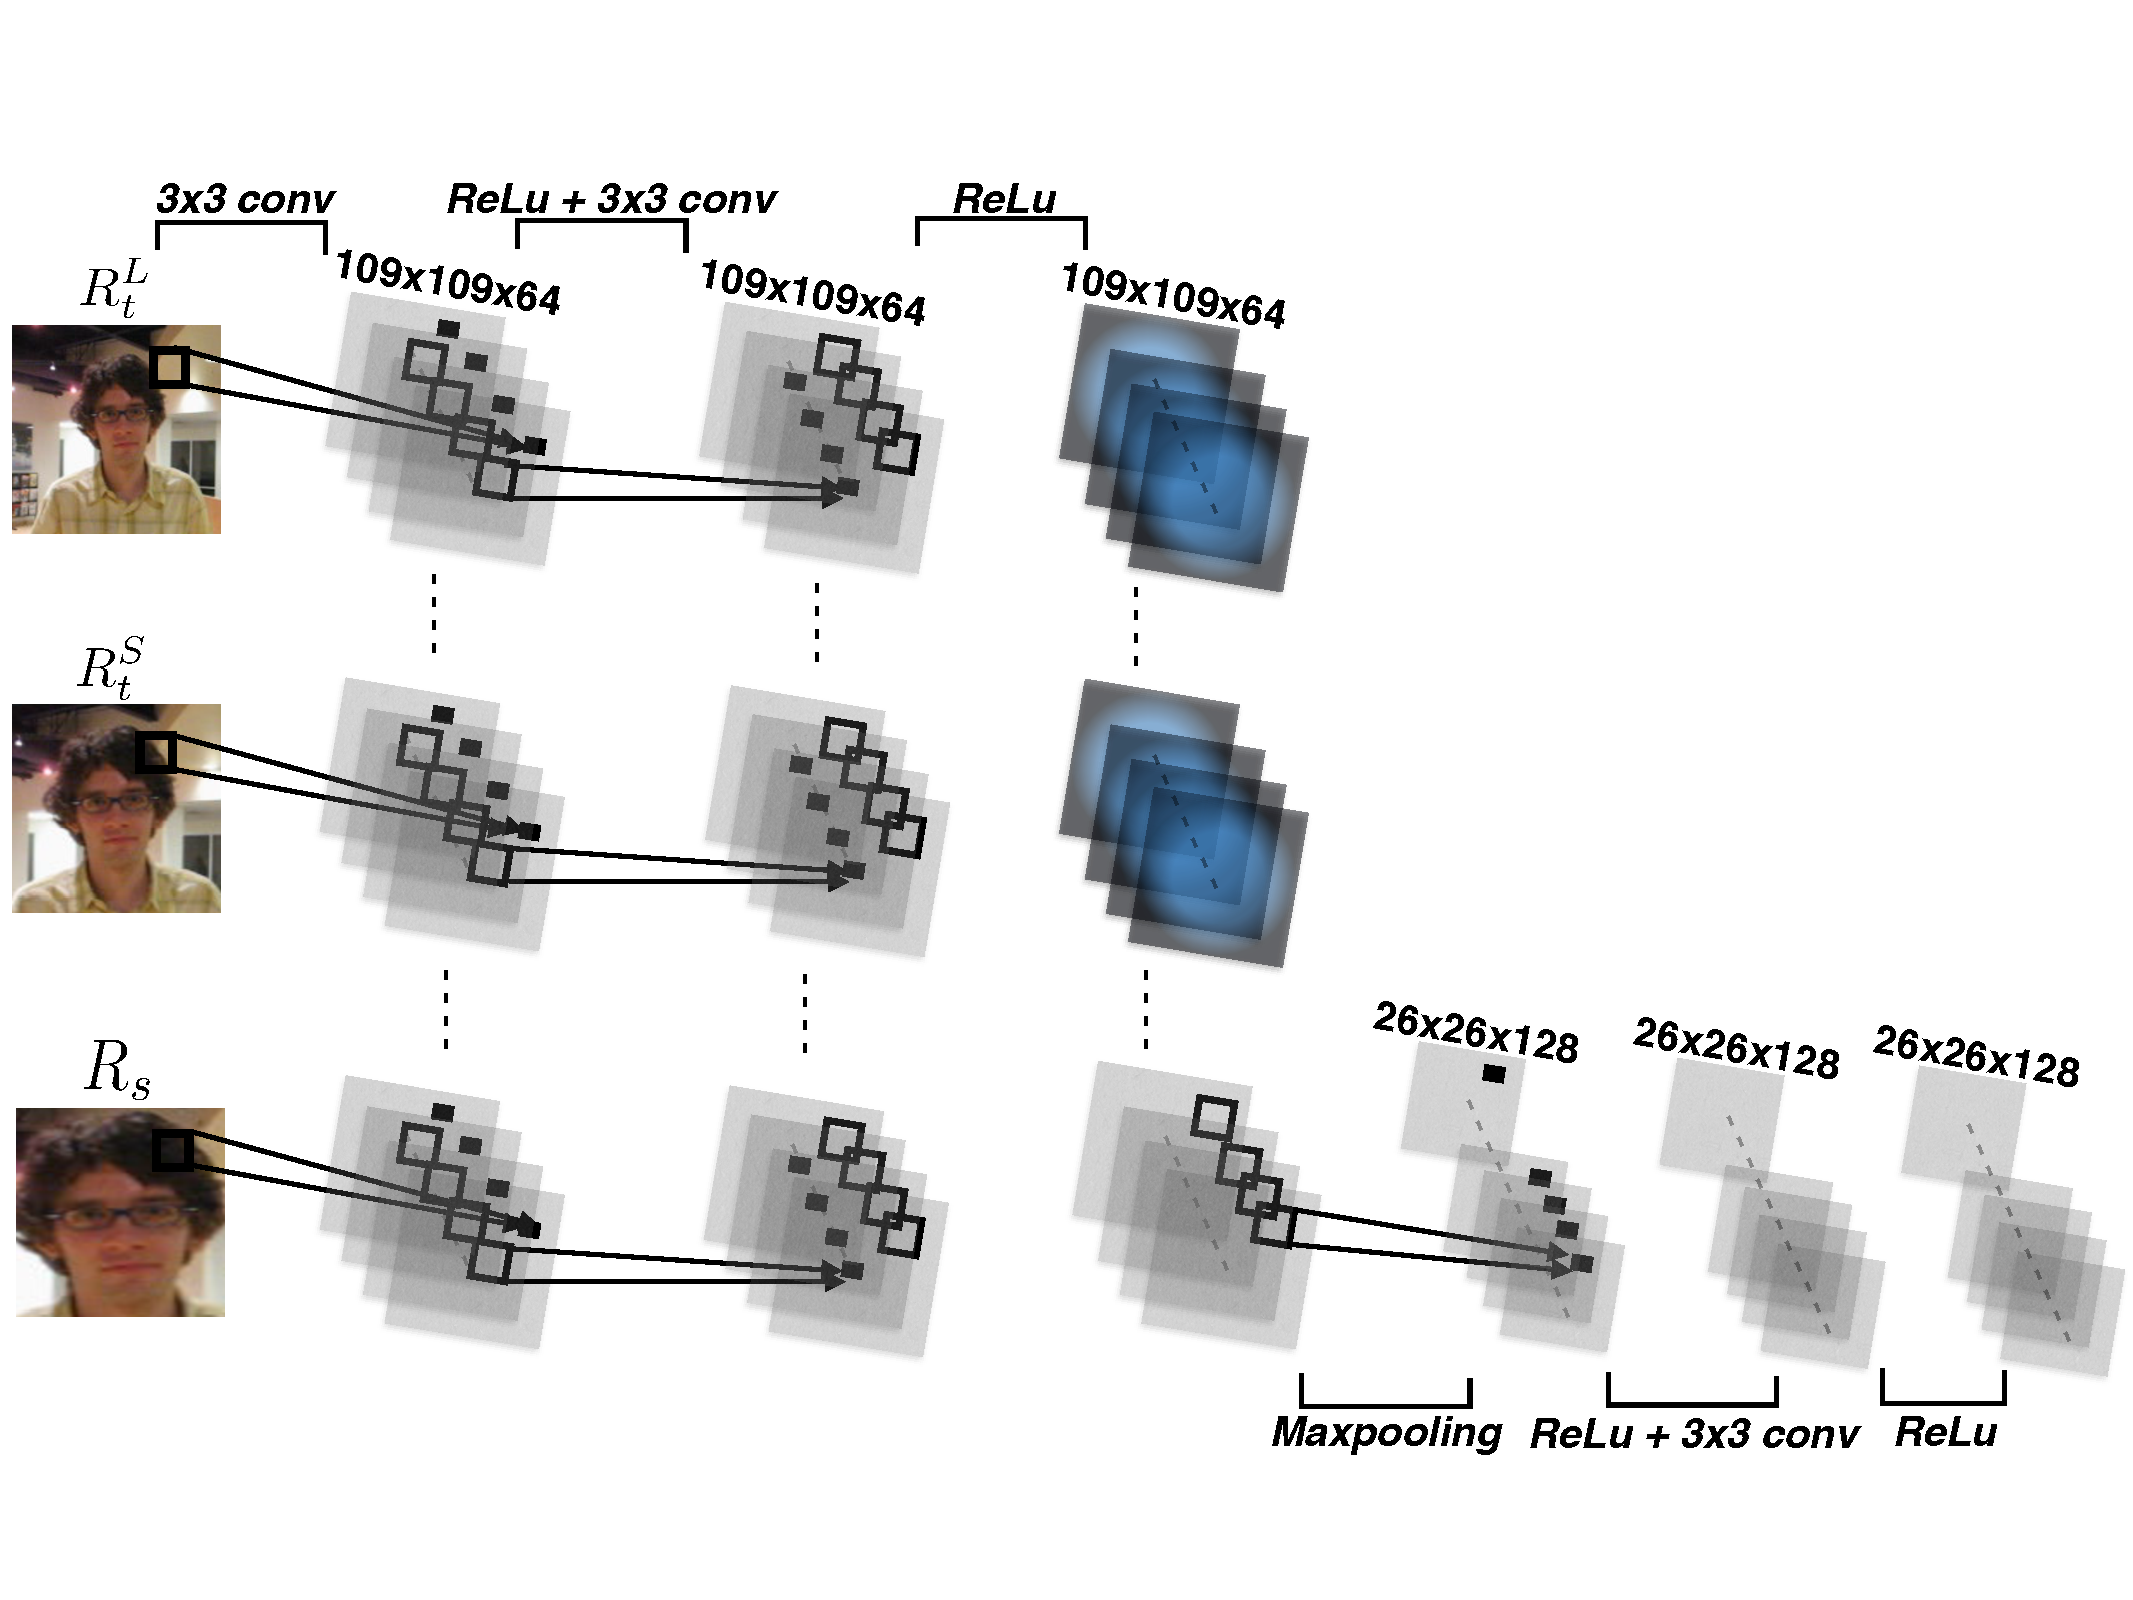
\includegraphics[width=0.48\textwidth]{./figures/Filters_Details_CNN.pdf}
\caption{The proposed conv224-VGGNet feature extraction in Deep{\it
    E}nKCF. $R_{t}^{L}$ and $R_{t}^{s}$ used an hanning window to
  avoid distortion caused by FFT operation whereas $R_{s}$ does not,
  in order to avoid target boundary information loss.}
\label{fig:Filters_CNN}
\end{figure}

\textbf{Particle Filter for Smoothing Transition among KCFs}
\begin{comment}
{\it Burak: Does what this section explains still hold good? If what
  this section explains still makes sense, the translation filter,
  $R_{t}^{L}$ doesn't do a good job. Isn't it? If it's not, revise
  this section.}
  
  {\it YoungWoo : I did not understand what $R_{t}^{L}$ has to do with 
  particle filter}

{\it Burak: Earlier we told the readers why we wanted to have two
  translation filters: one for smaller region, $R_{t}^{S}$, and
  another for larger region, $R_{t}^{L}$. The reason why we have two
  translation filter, instead of one because we wanted to minimize any
  drifts, yes? Read the line from 354 to 374. Then if we say again
  here we have a particle filter for smoothing transition among KCFs,
  they might think those two translation filters do not do their jobs
  well?}
  
{\it YoungWoo : Particle filter smoothen the translations in between the
transitions. We want to reduce drifts from scale filter by having $R_{t}^{L}$, and
we want to reduce drifts from $R_{t}^{L}$ by having $R_{t}^{S}$. The particle filter
on the other hand aims at reducing the drifts and jumps further by bringing in the 
motion information.}
\end{comment}  
As explained earlier, the {\it E}nKCF updates a target's translation
at every other $k$ frames, particularly for estimating the target's
scale. Although the strategy of updating every other $k$th frames will
result in an optimal run-time performance, this may lead drifts at the
later frames. To prevent such potential drifts, we developed a Bayes
filter that incorporates a target's motion to smooth any intermediate
outputs from individual KCFs. In particular, we use a particle filter
to estimate the target's image coordinate based on the {\it E}nKCF's
outputs. The state in this paper, $\mathbf{X_t}$, represents the target's pixel
coordinates and its velocity, $\mathbf{X_t} = \lbrace x, y, v_{x}, v_{y}
\rbrace$, where $x$ and $y$ are the pixel coordinates of the target's
centroid, $v_x$ and $v_y$ are the velocity estimated along the
$x$-axis and $y$-axis. The particle filter predicts, using a constant
velocity motion model, a target's next state by generating a predefined
number of particles. Then it uses the confidence maps of {\it E}nKCF
as observation to update the state. The weight of a particle is
computed as, $w_{p_{t}}(x_{t},y_{t}) = \sum_{i=1}^{N}\sum_{j=1}^{M} \mathbf{y_{R}}(x_{t}-i,y_{t}-j)$,
where $w_{p}$ denotes the weight of the particle $p$ at time $t$, and $N$ and $M$ denote the
size of rows and columns of the confidence map. 
%Alternatively one can
%also use the Euclidean distance of particles to the location of
%maximum response of the confidence map.
\begin{comment}
We chooses some particles based on their importance to estimate the
target's next state, i.e., its pixel coordinates as $\hat{X}_{t} =
\sum_{p=1}^{P}w_{p_{t}} X_{t}.$ Note that, unlike a typical operation
of a particle filter, we skip the importance re-sampling step when the
scale filter, $R_{s}$, estimates the target's scale change. This is
because we observe the confidence map from the scale filter, $R_s$ is
sometime noisy. In addition, at every iteration, we check the variance
in the velocity components of the particles to re-assign velocities
from uniform initial distribution to keep variance high enough.
\end{comment}

%----------------------------------------------------------------------
\section{Experiments} \label{sc:Experiments}
%---------------------------------------------------------------------- 
We evaluate, using the object tracking benchmark datasets, the
performance of the proposed algorithm {\it E}nKCF and its variants.
Particularly, we choose two publicly, available datasets:
OTB100\footnote{\url{http://cvlab.hanyang.ac.kr/tracker_benchmark/benchmark_v10.html}}
and
UAV123\footnote{\url{https://ivul.kaust.edu.sa/Pages/Dataset-UAV123.aspx}}\cite{mueller2016uav123}.
The OTB100 dataset is comprised of the videos about 100 objects
whereas UAV123 dataset contains aerial footages of 123 objects.  We
first evaluate the performance of {\it E}nKCF with two hand-crafted
features, fHoG and color-naming.  With this version, we would like to
have an object tracking algorithm that ``efficiently'' runs on an
embedded system, a drone, for example, in ``high speed,'' $\ge 30$
fps. Given this, we believe that the UAV123 dataset is a good fit in
evaluating the performance of the proposed algorithm. In addition, in
the UAV123 dataset, there are many challenging, realistic scenes,
e.g., abrupt scale/illumination changes. Although we are primarily
interested in developing an algorithm for mobile, embedded robotic
applications, it is also important to compare the performance of the
proposed algorithm with those of the state-of-the-art in a nominal
dataset. To this end, we chose the OTB100 dataset that contains the
videos recorded from smart phones and typical cameras in perspective
view. Also, we tested the proposed algorithm on a temporally
down-sampled version of the UAV123 dataset, called UAV123$\_$10fps
dataset. What we would like to evaluate using this modified dataset is
how robust the proposed algorithm is to the drastic motions of camera
and targets. Finally, we evaluate the Deep{\it E}nKCF, {\it E}nKCF
with deep features, on the UAV123 dataset to observe how much gain we
can achieve over hand-crafted features.

\textbf{Finding Optimal Hyper-parameters} As each of three KCFs in
       {\it E}nKCF is designed to address specific challenges in
       single target tracking problem, the optimal parameters for
       individual KCFs should be different. We set the learning rates
       of individual filters, $R_{t}^{L}$, $R_{t}^{S}$, and $R_{s}$
       differently as $0.020$, $0.020$ and $0.010$. For the kernel of
       the Gaussian neighboring function, we empirically found the
       optimal values of $\alpha$ as $0.7$, $0.6$, and $0.9$ for
       $R_{t}^{L}$, $R_{t}^{S}$, and $R_{s}$. We set the scale filter
       update threshold, $T_{R_{s}}$, to 4, peak-to-sidelobe (PSR)
       ratio. The padding size for the correlation filters is tuned to
       $3$ for $R_{t}^{L}$, $2.50$ for $R_{t}^{S}$, and $1$ for
       $R_{s}$. For our particle filter implementation, we empirically
       set the number of particles to $1,000$ to balance the run-time
       performance and accuracy. To keep the level of variance among
       the particles reasonable, we performed the re-sampling only
       when the \textit{efficient number of samples}, ($ \hat{N}_{eff}
       \approx (\sum_{p=1}^{P}\mathbf{w}_{p}^{2})^{-1} $), is lower than a
       pre-defined threshold.

\begin{figure*}[h]
\centering
\begin{tabular}{ccc}
\tiny\quad\textbf{UAV123}\hspace{.37\linewidth}\textbf{OTB100}\\
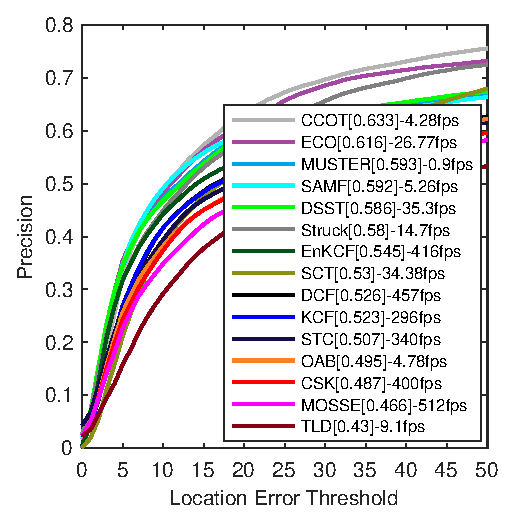
\includegraphics[width=3.30cm]{./figures/pr_uav123.eps}
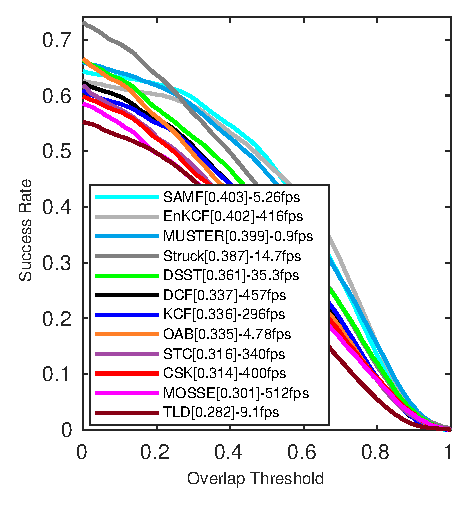
\includegraphics[width=3.55cm]{./figures/sr_uav123.eps}
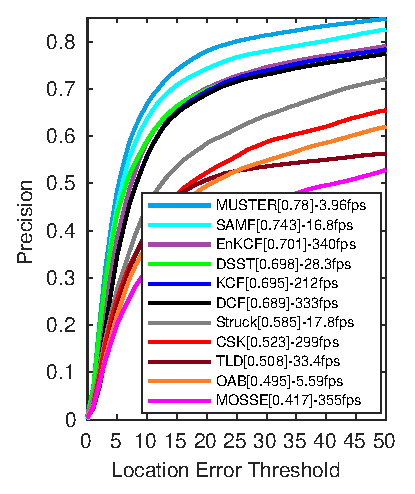
\includegraphics[width=3.30cm]{./figures/pr_otb100.eps}
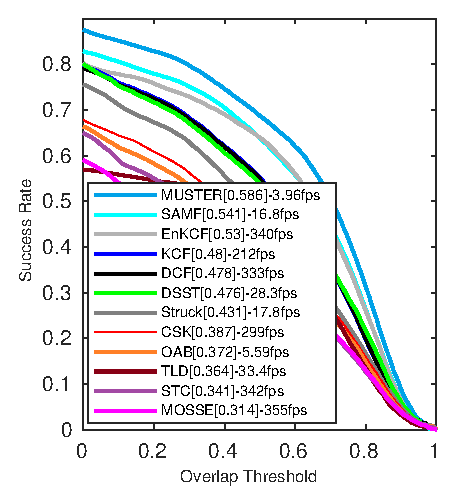
\includegraphics[width=3.55cm]{./figures/sr_otb100.eps}\\
\end{tabular}
\caption{Comparison of {\it E}nKCF's performance with other trackers on the UAV123 and OTB100 datasets.}
\label{fig:UAV123_DATASET}
\end{figure*}

%\textbf{Features Selections} We used different features for each of
%three KCFs as each of them has different goals to accomplish. In
%particular, the translation filter, $R_{t}^{L}$, uses both the fast
%Histograms of Oriented Gradients (fHoG) \cite{felzenszwalb2010object}
%and color-naming \cite{van2009learning} features to more effectively
%learn the background around the target as shown in Figure \ref{fig:Filters}. 
%Through experiments, we found that only fHoG didn't work well to cover a larger ROI; another
%translation filter, $R_{t}^{S}$, worked well when it used fHoG
%features only; the scale filter, $R_{s}$ did when it used both fHoG
%and color features.

\textbf{Performance on UAV123 Dataset} We used the precision and
success rate to compare the performance of the proposed algorithm with
those of the state-of-the-art, online algorithms for high speed
tracking. For the precision, we rank the trackers based on the
precision numbers at 20 pixels whereas in the success rate plots,
trackers are ranked based on area under curve (AUC) scores. The
tracking algorithms under the comparison include ones in high-speed
($\geq$300 fps): KCF \cite{henriques2015high}, CSK
\cite{henriques2012exploiting}, DCF \cite{henriques2015high}, MOSSE
\cite{bolme2010visual}, and STC \cite{zhang2014fast}
and ones in relatively lower-speed ($\geq$50): ECO \cite{DanelljanCVPR2017}, 
CCOT \cite{DanelljanECCV2016}, SCT \cite{Choi_2016_CVPR}, SAMF
\cite{li2014scale}, DSST \cite{danelljan2014accurate}, Struck
\cite{hare2012efficient}, MUSTER \cite{hong2015multi}, TLD
\cite{kalal2012tracking}, and OAB \cite{zhang2012robust}. Figure
\ref{fig:UAV123_DATASET} shows the results on the UAV123 dataset. {\it
  E}nKCF outperformed most of the high-speed tracking methods by
$3\%$-$15\%$ at 20 pixels precision. Three algorithms, SAMF, DSST, and
Struck did about 5\% better than ours in accuracy, but 10-20 times
slower. For the scale adaptation, {\it E}nKCF did second best in terms
of AUC for the success rate plot. It outperformed other tracking
methods in high-speed by about $20\%$-$25\%$ in AUC. In addition, it
performed even better than those algorithms that are slow, but a
slightly better in precision. For example, for AUC, {\it E}nKCF
outperformed Struck and DSST by $5\%$ and $10\%$ while running at more
than $10$ and $30$ times faster.

\begin{table*}[!h]
\smaller
\begin{center}
\color{green}--- Best \hspace{.15\linewidth}\color{red}--- $2^{nd}$ Best \hspace{.15\linewidth}\color{blue}--- $3^{th}$ Best \color{black}\\
\resizebox{\textwidth}{!}{\begin{tabular}{|l|c|c|c|c|c|c|c|c|c|}
\hline
Method & {\it E}nKCF & $R_{t}^{S}$+$R_{t}^{L}$+$R_{s}$ & $R_{t}^{L}$+$R_{s}$ & $R_{t}^{S}$+$R_{s}$ & $R_{t}^{L}$* & $R_{t}^{S}$* & $R_{t}^{L}$+$R_{s}$* & $R_{t}^{S}$+$R_{s}$* & $R_{t}^{L}+R_{t}^{S}$+$R_{s}$* \\
\hline\hline
Pr. ($20$px) & \color{blue}53.9 & 48.93 &52.41 & 48.10 & 51.88 & 51.29 & \color{red} 55.85 & 52.14 & \color{green}58.16 \\
SR ($50\%$) & \color{red} 40.2 & 36.75 & 38.23 & 36.04 & 35.12 & 34.43 & \color{blue}39.89 & 38.51 & \color{green}41.58 \\
FPS & \color{red} 416 & \color{blue}412 & 370 & \color{green}425 & 365 & 384 & 135 & 151 & 99 \\
\hline
\end{tabular}}
\end{center}
\caption{Results of running different combinations of the KCFs for
  UAV123 dataset.  The '$*$' represents
  sequential approach where multiple KCFs are run in the given order in every frame as in LCT \cite{ma2015long}.}
\label{table:Comparison_to_LCT}
\end{table*}

\textbf{Finding Optimal Combination and Deployment Order of Multiple
  KCFs} In addition to the comparison with other tracking methods, we
also conducted an experiment to see what combination and deployment
order of the KCF work best. Table \ref{table:Comparison_to_LCT}
presents results of this experiment. For this experiment, we did not
use the particle filter to evaluate which order would work best,
without any extra components. The method at the $2^{nd}$ column
flipped the order of deploying $R_{t}^{L}$ and $R_{t}^{S}$. The one at
the $3^{th}$ column removed $R_{t}^{S}$ and replaces with $R_{t}^{L}$
whereas the one at the $4^{th}$ column removes $R_{t}^{L}$. The
methods marked with ``*'' ran the filters on every frame in the listed
order. The methods at the $7^{th}$ and $8^{th}$ columns ran a
translation and a scale filter on every frame which is very similar to
the way the LCT tracker \cite{ma2015long} runs.\footnote{To be
  precise, the LCT tracker comes with a re-detection module for a
  long-term tracking.} In short, we empirically verified that
\textit{E}nKCF is an optimal way of using multiple KCFs, in terms of
tracking accuracy and run-time performance. For example, we could
achieve 4.26\% higher in accuracy by running $R_{t}^{L}$ and $R_{S}$
at every frame, but this combination decreases run-time performance to
317 fps. Lastly, we run $R_{L}$, $R_{t}^{S}$ and $R_{s}$ in every
frame where $R_{t}^{S}$ uses the translation estimated by $R_{t}^{L}$
to update translation and $R_{s}$ uses the final translation
estimation given by $R_{t}^{S}$ to update the scale. Table
\ref{table:Comparison_to_LCT} indeed showed that it is very useful to
deploy more than one KCF as long as the deployment order is optimal.

\textbf{Evaluation on Particle Filter Contribution} For the UAV123
dataset, we also evaluated the performance of the {\it E}nKCF with and
without the particle filter. In particular, we use 50 sequences
labeled as no abrupt camera motion in the dataset. To evaluate the
robustness of particle filter, we add noise, drawn from a uniform
distribution ($[-20,20]$), to the translation estimations of the
KCFs. In these setup, the {\it E}nKCF with particle filter achieves
$51.98\%$ precision ($20$px), outperforming the one without particle
filter {\it E}nKCF by $6.32\%$. Thus, with the removal of global
camera motion, the integration of particle filter into the {\it E}nKCF
as shown in Figure \ref{Workflows} further improved the results.

\textbf{Performance on OTB100 Dataset} Figure \ref{fig:UAV123_DATASET}
shows the results on the OTB100 dataset. Same as with UAV123 dataset,
we observed a similar performance. In particular, {\it E}nKCF showed a
good performance for handling the scale changes. It was the third best
and the second fastest tracking algorithm. For the precision metric,
{\it E}nKCF performed slightly better than most of tracking algorithms
in high-speed trackers. Interestingly, it outperformed another
correlation filter based tracker, DSST, but performing $5\%$ behind of
another low-speed scale adaptive SAMF tracker.

\textbf{Performance on UAV123$\_$10fps Dataset} It maybe a slight
digression from the main idea -- the idea of deploying multiple KCFs
to make a very fast and effective, single target tracking
available. We found that, with a slight modification, the proposed
method can effectively handle tracking of object in fast motion and in
large camera motion. Specifically, we modified {\it E}nKCF by running
$R_{t}^{L}$ every frame and remove the particle filter instead. We
tested this modified {\it E}nKCF with another vision of the UAV123 that
the original dataset was temporally down-sampled at $10$ fps and makes
the challenging original dataset, because of objects in fast motion
and large ego-motion, more challenging. This is because the magnitude
of those motions is even bigger. Figure \ref{fig:UAV123_10fpsDATASET}
compares the performance of the modified version of {\it E}nKCF and
other tracking methods. Our tracker outperforms other high-speed
correlation filter based trackers including KCF, DSST by about
$15\%$-$20\%$ and showed a precision rate similar to that of SAMF. On
the other hand, it does decent job in scale estimation. It ranks as
second in AUC while running about $150$ faster than MUSTER.

\begin{figure}[!h]
\centering
\begin{tabular}{cc}
\tiny\quad\textbf{UAV123$\_$10fps}\\
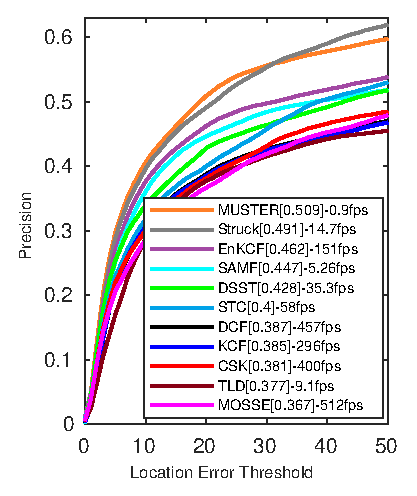
\includegraphics[width=3.30cm]{./figures/pr_uav123_10fps.eps}
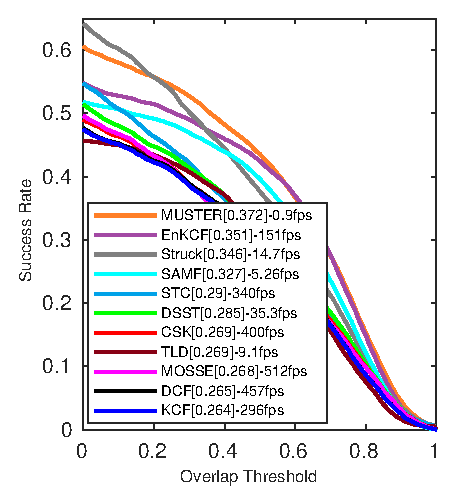
\includegraphics[width=3.55cm]{./figures/sr_uav123_10fps.eps}\\
\end{tabular}
\caption{Comparison of a modified {\it E}nKCF's performance with those
  of the state-of-the-art tracking algorithms on the UAV123$\_$10fps
  dataset where the original UAV123 data was temporally downsampled.}
\label{fig:UAV123_10fpsDATASET}
\end{figure}

\textbf{Evaluation with Deep Features} Our focus so far was to build a
high speed tracker that can run at $30$fps on a single-board, embedded
system. To this end, we used two conventional features, fHoG and
color-naming for the {\it E}nKCF. At the same time, we observed that
the feature vectors learned from a CNN have been used to improve the
performance of the trackers based on KCF \cite{ma2015hierarchical,
  danelljan2015convolutional}, and some of the single-board, embedded
systems have GPUs. We believe that the performance of the {\it E}nKCF
could be also improved with deep convolutional features trained on ImageNet dataset.
\begin{comment}
{\it Burak: I'm not sure what you wanted to say with ``Deep Learning
  Features.'' My edit stopped at the above paragraph because I got
  confused. At least you'll have to explain the point of adding this
  section.

  I don't know why Figure 7 is presented separately from Figure 5. If
  you want to keep this way, you need, at least, to have their scales
  same -- precision should have the same range, say 0.8 as the max
  value.

  YoungWoo : The point of adding this section is to evaluate the
  same tracker with deep features (CNN) and see how much accuracy improvement
  we get. However, I tried to highlight that, by employing deep features
  the targeted embedded system changes from low-end (CPU-only) to 
  higher-end system (GPUs). The two papers I cited employs the features
  from the first several layers of the VGGNet. This is a common practice
  in supporting the trackers with CNN features. 

  Burak: I'm not saying what you did -- use CNN features to feed an
  online tracker. Yes, many people did such before. My worry is to
  make our paper look a christmas tree -- a paper w/ too many stuffs
  to evaluate under a certain theme. And, adding these new stuffs
  along the way of preparing any submissions continuously asks us to
  rewrite this paper from the top to all the way down. We need to
  focus on a certain idea when to submit a paper to a
  conference. Adding a bit more meats and stuffs to the main idea is
  usually done in a journal paper.

  If I add this to figure 5, it does not make sense, because all the
  trackers we compare, use hand-crafted features and run on CPU. For
  this reason, I wanted to compare EnKCF with deep features
  (higher-end system) and hand-crafted features (low-end system).

  Burak: Given what we agreed upon what you did, I think you can still
  put them together in that we're comparing different versions of
  apples, not orange, under the same criterion. Think about it.
 
  The figure 7(a) and figure 5 have almost the same range (0,73 and 0.70)
  I will update the figure 5 to have 0.73 range as well. I test the EnKCF
  with CNN features only on the UAV123 dataset.

  Burak: We don't expect the reviewers or readers to exactly see what
  we saw here. Keep their scales same -- whatever maximum value you
  choose for the y-axis for one graph, use the same scale to all other
  same graphs.}
\end{comment}

Figure \ref{fig:UAV123_DATASET_DeepFeatures} shows DeepE{\it n}KCF's
performance on UAV123 dataset. Deep{\it E}nKCF outperformed the {\it
  E}nKCF with hand-crafted features by about $3\%$ to $5\%$ in
precision (20 px) and $2\%$ in success rates (AUC). The
\textit{conv224-VGG} setting performed slightly better than
\textit{conv222-VGG} in precision while achieving similar success rate
(AUC). This indicates that higher level feature abstraction works
better for the smaller ROIs. By using feature abstractions from the
VGGNet pre-trained on millions of images, we can better represent the
low level features of the object than hand-crafted features in
challenging cases such as low contrast ROIs. However, we believe that
the contribution of the deep features is limited by two factors: (1)
low spatial resolution in deeper layers and (2) lost targets due to
large target and camera motion in the UAV123 dataset.

\begin{comment}
{\it Burak: You'll have to explain 1) why, you think, DeepEnKCF worked better, 2) 
why DeepEnKCF didn't perform a way better than EnKCF, 3) why did conv224-VGG perform better than conv222-VGG.}
\end{comment}
\begin{figure}[!h]
\centering
\begin{tabular}{ccc}
\tiny\quad\quad\textbf{UAV123}\\
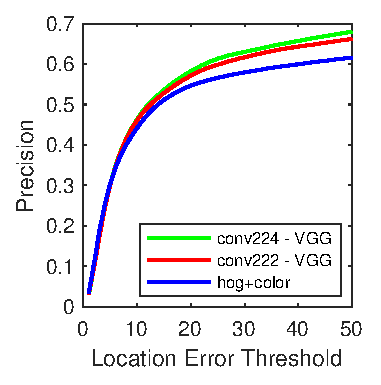
\includegraphics[width=3.60cm]{./figures/pr_deep.eps}
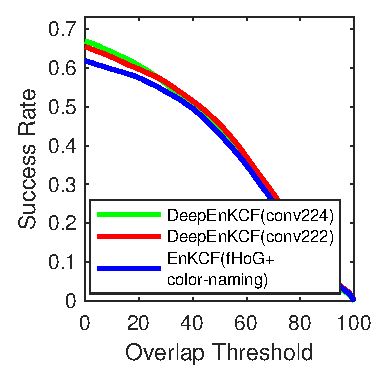
\includegraphics[width=3.70cm]{./figures/sr_deep.eps}\\
\end{tabular}
\caption{Comparison of {\it E}nKCF's ({\it fHoG} + {\it color-naming}) performance with Deep{\it E}nKCF on the UAV123
dataset.}
\label{fig:UAV123_DATASET_DeepFeatures}
\end{figure}

%\begin{figure}[!h]
%\centering
%\begin{tabular}{ccc}
%\bmvaHangBox{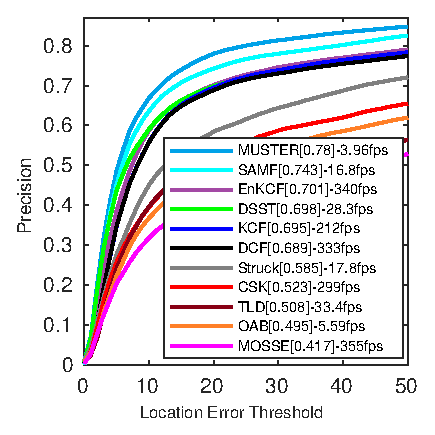
\includegraphics[width=3.30cm]{./figures/Precision_OTB100.eps}}
%\bmvaHangBox{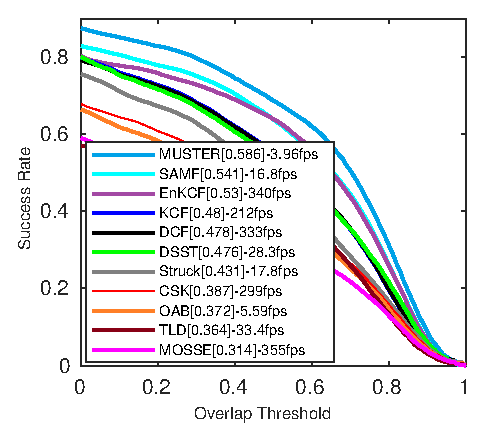
\includegraphics[width=3.80cm]{./figures/Success_OTB100.eps}}\\
%\end{tabular}
%\caption{Comparison of {\it E}nKCF's performance with those of the
%  state-of-the-art tracking algorithms on the OTB100 dataset.}
%\label{fig:OTB100_DATASET}
%\end{figure}

%\begin{table}
%\smaller
%\begin{center}
%\begin{tabular*}{\textwidth}{|l|c|c|c|c|c|c|c|c|}
%\hline
% & $R_{t}^{L}$+$R_{t}^{S}$+$R_{s}$ ({\it E}nKCF) & $R_{t}^{L}$+$R_{s}$ & $R_{t}^{S}$+$R_{s}$ & $R_{t}^{L}$ & $R_{t}^{S}$ & LCT  $R_{t}^{S}$+$R_{s}$ & LCT  $R_{t}^{L}$+$R_{s}$ & LCT  $R_{t}^{L}+R_{t}^{S}$+$R_{s}$\\
%\hline\hline
%Pr. ($20$px) & \textbf{53.9} & 48.09 & 52.50 & 51.88 & 51.29 & 52.14 & &  \\
%SR ($50\%$) & \textbf{40.2} & 36.04 & 37.85 & 35.12 & 34.42 & 38.51 & & \\
%FPS & 416 & 370 & 425 & 367 & \textbf{490} & 151 & & \\
%\hline
%\end{tabular*}
%\end{center}
%\caption{Evaluations of the different combinations of the proposed KCFs in UAV123 dataset. We decouple the re-detection module of the LCT tracker as we focus on the comparison of the multiple correlation filter framework between LCT and  {\it E}nKCF. $R_{t}^{S}$ and $R_{s}$ are used as proposed in
%\cite{ma2015long}, however, only three scale candidates ($1.02$, $1.00$, $1.00/1.02$) are used to perform realistic comparison. In the original paper, 33 scales with scale factor 1.02 is considered, resulting in low fps ($\leq50$fps).} 
%\end{table}

%---------------------------------------------------------------------- 
\section{Conclusion} \label{sc:Conclusion}
%---------------------------------------------------------------------- 
Running a computer vision algorithm on any existing embedded systems
for real-world applications is economically and practically very
attractive. To make such pipelines more plausible, however, those
algorithms should run faster with small footprint of computation
resource consumption. To make an object tracking algorithm meet these
practical requirements, we proposed an extension of KCF that
essentially deploys three KCFs, in turn, to address the scale change
and dynamic maneuvers of a target. The way we ran three KCFs is
optimal in a sense that efficiently handled the scale change and
effectively learned the translation of the target. We also developed a
Bayes filter, particle filter, to smooth the transition between three
KCFs. In particular, the particle filter estimated the target’s pixel 
coordinates using evolution of the target’s motion observed over frames.
Two public datasets were used to evaluate the performance of the
proposed algorithm and found, on average, the performance of the
proposed algorithm is better than those of the existing ones over 5\%
on precision at 20 pixels and 10-20\% on AUC on average. Our
implementation ran at 340 fps for OTB100 and at 416 fps for UAV123
data that is faster than DCF (292 fps) for OTB100 and KCF (292 fps),
DCF (457 fps) for UAV123. Finally, we encoded objects with deep
features to boost tracking performance by $5\%$ on embedded systems
with GPUs.

As future work, we investigate a way of re-initializing a target when
the target is lost, due to occlusion, illumination change, drastic
camera motion, etc.

{\small
\bibliographystyle{ieee}
\bibliography{draft}
}

\end{document}
